\def\year{}\relax
%File: formatting-instruction.tex
\documentclass[letterpaper]{article} %DO NOT CHANGE THIS
\usepackage{aaai20}  %Required
\usepackage{times}  %Required
\usepackage{helvet}  %Required
\usepackage{courier}  %Required
\usepackage{url}  %Required
\usepackage{graphicx}  %Required
\frenchspacing  %Required
\setlength{\pdfpagewidth}{8.5in}  %Required
\setlength{\pdfpageheight}{11in}  %Required
%PDF Info Is Required:
\pdfinfo{
/Title (Debiasing)
/Author (Xiaojie Wang)}
\setcounter{secnumdepth}{2}

\usepackage{balance} % balance references
\usepackage{booktabs} % professional table
\usepackage{threeparttable} % table footnote


\usepackage[ruled,linesnumbered,noend]{algorithm2e}
\usepackage{amsmath} % DeclareMathOperator
\usepackage{amsfonts} % mathbb
\usepackage{amssymb} % intercal
\usepackage{bm} % bm
\usepackage{enumitem} % enumerate
\usepackage{float} % pack figure
\usepackage{mathtools} % smashoperator
\usepackage{multirow} % multirow
\usepackage{stmaryrd} % llbracket
\usepackage{subcaption} % subfigure
\usepackage[hang,flushmargin]{footmisc} % footnote indent

%% operator
\def\stopgrad{\ensuremath{\bot}}
\newcommand{\transpose}{\mathsf{T}}
\newcommand{\matrixize}[1]{\mathbf{#1}}
\newcommand{\vectorize}[1]{\bm{#1}}
\newcommand{\lrdense}[2]{\smashoperator[lr]{#1_{#2}}}
\newcommand{\ldense}[2]{\smashoperator[l]{#1_{#2}}}
\newcommand{\rdense}[2]{\smashoperator[r]{#1_{#2}}}
\newcommand{\defeq}{\vcentcolon=}
%% math
\newcommand{\realNumber}{\mathbb{R}}
%% user
\newcommand{\nUser}{M}
\newcommand{\iUser}{m}
%% item
\newcommand{\nItem}{N}
\newcommand{\iItem}{n}
%% pair
\newcommand{\allPairs}{\mathcal{A}}
\newcommand{\obsPairs}{\mathcal{O}}
\newcommand{\misPairs}{{\lnot\mathcal{O}}}
\newcommand{\obsBiasedPairs}{\mathcal{B}}
\newcommand{\misBiasedPairs}{{\lnot\mathcal{B}}}
\newcommand{\obsUnbiasedPairs}{\mathcal{U}}
\newcommand{\misUnbiasedPairs}{{\lnot\mathcal{U}}}
%% propensity
\newcommand{\propensity}{p_{u,i}}
\newcommand{\estimatedPropensity}{\hat{p}_{u,i}}
%% rating
\newcommand{\trueRatings}{\matrixize{R}}
\newcommand{\biasedRating}{r_{u,i}}
\newcommand{\unbiasedRating}{r_{v,j}}
\newcommand{\imputedRating}{\hat{r}_{u,i}}
\newcommand{\ratingScale}{r}
\newcommand{\nScale}{R}
%% observation
\newcommand{\observations}{\matrixize{O}}
\newcommand{\obsIndicator}{o}
\newcommand{\observation}{\obsIndicator_{u,i}}
%% feature
\newcommand{\nFeature}{K}
\newcommand{\iFeature}{k}
\newcommand{\iFeatures}{\mathcal{X}}
\newcommand{\allFeatures}{\matrixize{X}}
\newcommand{\featureMark}{x}
\newcommand{\biasedFeatures}{\vectorize{\featureMark}_{u,i}}
\newcommand{\unbiasedFeatures}{\vectorize{\featureMark}_{v,j}}
\newcommand{\feature}{\featureMark_{u,i,\iFeature}}
%% objective
\newcommand{\likelihood}[1]{\mathcal{F}_{\rm #1}}
\newcommand{\loss}[1]{\mathcal{L}_{\rm #1}}
\newcommand{\inaccuracy}[1]{\mathcal{I}_{\rm #1}}
\newcommand{\obsLoss}{\ell}
\newcommand{\misLoss}{\ell}
\newcommand{\innerMark}{I}
\newcommand{\outerMark}{O}
\newcommand{\varianceMark}{SV}
\newcommand{\rOuterMark}{RO}
%% naive bayes
\newcommand{\nbProbability}{p}
\newcommand{\nbObservation}{\nbProbability}
\newcommand{\nbCondition}{\nbProbability}
\newcommand{\nbRating}{\nbProbability}
%% logistic regression
\newcommand{\lgBias}{b}
\newcommand{\lgWeight}{\vectorize{w}}
%% neural propensity
\newcommand{\nEmbedding}{E}
\newcommand{\sLayer}{L}
\newcommand{\nLayer}{D}
\newcommand{\iLayer}{d}
\newcommand{\npLinearBias}{\lgBias}
\newcommand{\npLinearWeight}{\lgWeight}
\newcommand{\npDeepBias}{\vectorize{b}}
\newcommand{\npDeepWeight}{\matrixize{W}}
\newcommand{\npLastLayer}{\vectorize{w}_\nLayer}
\newcommand{\npOnlyLayer}{\vectorize{w}_0}
\newcommand{\npEmbeddings}{\matrixize{Z}}
\newcommand{\npEmbedding}{\vectorize{z}}
\newcommand{\npNonZero}{\vectorize{n}_{u,i}}
\newcommand{\npSecondOrder}{\vectorize{s}}
\newcommand{\npConcatenated}{\vectorize{c}_{u,i}}
\newcommand{\npAugmented}{\hslash} % {\text{MLP}}
%% rating model
\newcommand{\ratingName}{y}
\newcommand{\ratingParam}{\phi}
\newcommand{\ratingModel}{\ratingName_\ratingParam(\biasedFeatures)}
%% error model
\newcommand{\errorName}{g}
\newcommand{\errorParam}{\xi}%{\psi}
\newcommand{\errorModel}{\errorName_\errorParam(\biasedFeatures)}
\newcommand{\trueError}{e_{u,i}}
\newcommand{\lossName}{s}
\newcommand{\trueLoss}{\lossName_\ratingParam(\biasedFeatures)}
\newcommand{\imputedLoss}{\hat{\lossName}_\ratingParam(\biasedFeatures)}
%% propensity model
\newcommand{\propensityName}{q}
\newcommand{\propensityParam}{\theta}
\newcommand{\propensityModel}{\propensityName_\propensityParam(\biasedFeatures)}
%% algorithm
\newcommand{\parameters}{\rho}
\newcommand{\regularization}{\lambda}
\newcommand{\textalg}[1]{\texttt{\textsc{#1}}}
\newcommand{\nStep}{S}
\newcommand{\step}{s}
\newcommand{\learningRate}{\eta}
\newcommand{\nEpoch}{T}
\newcommand{\epoch}{t}

%% one-column table and figure
% \setlength{\textfloatsep}{20.0pt plus 2.0pt minus 4.0pt}
% \setlength{\floatsep}{12.0pt plus 2.0pt minus 2.0pt}
% \setlength{\intextsep}{12.0pt plus 2.0pt minus 2.0pt}
% \setlength{\textfloatsep}{10.0pt plus 1.0pt minus 2.0pt}
% \setlength{\floatsep}{6.0pt plus 1.0pt minus 1.0pt}
% \setlength{\intextsep}{6.0pt plus 1.0pt minus 1.0pt}
\setlength{\textfloatsep}{8.0pt plus 0.8pt minus 1.6pt}
\setlength{\floatsep}{4.8pt plus 0.8pt minus 0.8pt}
\setlength{\intextsep}{4.8pt plus 0.8pt minus 0.8pt}
%% two-column table space below
\setlength{\dbltextfloatsep}{10.0pt plus 1.0pt minus 2.0pt}
%% table and figure caption
% \setlength{\abovecaptionskip}{10.0pt plus 1.0pt minus 2.0pt}
\setlength{\abovecaptionskip}{4.0pt plus 0.4pt minus 0.8pt}
\captionsetup[subfigure]{aboveskip=0.6pt,belowskip=0.6pt}

\usepackage{caption}
\usepackage{subcaption}
\captionsetup{font=small}
% \captionsetup[sub]{font=scriptsize}
\captionsetup[sub]{font=small}
\captionsetup[figure]{name={Fig.}}

%% space between number and text in section titles
% \makeatletter
% \renewcommand*{\@seccntformat}[1]{\csname the#1\endcsname\hspace{0.1cm}}
% \makeatother

%% roman numeral
\makeatletter
\newcommand*{\myroman}[1]{\expandafter\@slowromancap\romannumeral #1@}
\makeatother

%% comments
\usepackage{xcolor}
\definecolor{red}{RGB}{255,0,0}
\newcommand{\comment}[1]{\textcolor{red}{\textbf{\small{[#1]}}}}

\begin{document}
% The file aaai.sty is the style file for AAAI Press 
% proceedings, working notes, and technical reports.
%

\title{LTD: Learning to Debias for Training Recommender Systems}
\author{}
\maketitle


\begin{abstract}
Datasets used to train recommender systems are usually biased, e.g., the propensities (or probabilities) of observing different ratings are not the same. To handle biased datasets, recent studies first estimate propensities by maximizing a likelihood function and then predict ratings by minimizing a propensity-weighted loss. Such an approach is vulnerable to the error and variance of propensity estimation, which may cause high recommendation inaccuracy. To address this issue, we propose learning to debias (LTD). It adopts a nested formulation to learn a propensity (estimation) model by directly minimizing the recommendation inaccuracy of a rating (prediction) model on an unbiased dataset. For the propensity model learned this way, all features of observed ratings can be used to estimate propensities. Hence, we propose using a neural architecture to effectively exploit these features. However, it is challenging to train the propensity and the rating model's parameters within LTD. To tackle this challenge, we apply back-propagation on a parameter update function of the rating model, and regularize the training with the sample variance of estimated propensities. We conduct extensive experiments on four real-world datasets. The experiments show that LTD significantly outperforms the state-of-the-art irrespective of using unbiased or biased datasets for evaluation.
% It nests learning a rating (prediction) model within learning a propensity (estimation) model by directly minimizing the recommendation inaccuracy on an unbiased dataset.
% To address this issue, we propose learning to debias (LTD), which learns a propensity (estimation) model by minimizing the recommendation inaccuracy of a rating (prediction) model on an unbiased dataset. 
% To tackle the challenge of training the propensity model, we approximate the best parameter values for the rating model with the current parameter values at each step of training.
% We overcome the difficulty in obtaining stable gradients to update the rating model by using the sample variance of the estimated propensities per mini-batch to regularize the training.
\end{abstract}


\section{Introduction}
Normally, datasets for training recommender systems are biased~\cite{wang2018modeling}.
For example, on music recommendation datasets, users often select to rate only songs that they like, and thus ratings to the other songs are often missing~\cite{ling2012response}.
Due to this self-selection by users, the propensity (i.e., probability) of observing a larger rating is usually also larger.
Existing studies show that ignoring such biasedness in rating observation and assuming uniform propensities will lead to high recommendation inaccuracy~\cite{marlin2007collaborative}.
This motivates the \emph{debiasing} problem, which aims to reduce the recommendation inaccuracy given biased datasets for training~\cite{marlin2009collaborative}.

Recent approaches solve this problem by two-phase learning, which is illustrated in Fig.~\ref{fig:two phase}~\cite{schnabel2016recommendations,wang2019doubly}:
(1) The \textbf{first} phase (see top half of Fig.~\ref{fig:two phase}) learns a propensity model to estimate propensities by maximizing a likelihood function.
(2) The \textbf{second} phase (see bottom half of Fig.~\ref{fig:two phase}) trains a rating model to predict ratings by minimizing a propensity-weighted loss.
The rating model trained this way may still have the issue of high recommendation inaccuracy.
This is because the two-phase learning is vulnerable to the error and variance of propensity estimation~\cite{schnabel2016recommendations}.
Specifically, the two-phase learning fixes and does not learn the propensity model during \emph{debiasing}, i.e., using the propensity model to train the rating model (see bottom half of Fig.~\ref{fig:two phase}).
Therefore, the error and variance of propensity estimation will propagate into the training of the rating model, and thus the resulting rating model may have a poor generalization ability~\cite{wang2019doubly}.
% have a loose generalization bound on its recommendation inaccuracy
Moreover, another issue is that when learning the propensity model, the likelihood function is irrelevant to the recommendation inaccuracy.
The propensity model learned this way is sub-optimal in the sense that it does not necessarily contribute to reducing the recommendation inaccuracy of the rating model (e.g., when evaluated on an unbiased dataset or when deployed for online services).
% reducing the error of the rating model.

\begin{figure}[!t]
\hspace*{-0.44cm}
\begin{minipage}[t]{1.090\linewidth}
\centering
\begin{figure}[H]
\centering
\begin{subfigure}{0.495\textwidth}
  \centering
  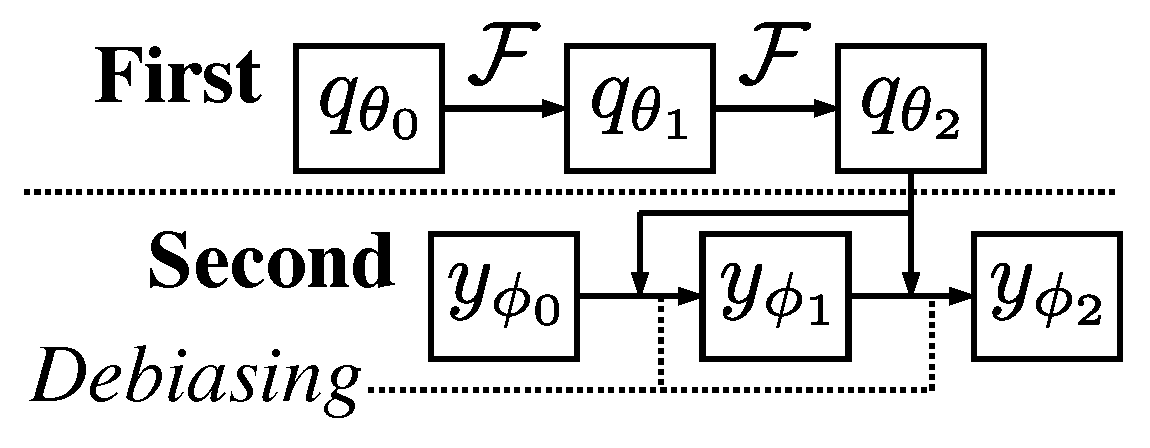
\includegraphics[width=4.2cm]{fig/two_phase.eps}
  \caption{Existing two-phase learning.}
  \label{fig:two phase}
\end{subfigure}
\hfill
\begin{subfigure}{0.495\textwidth}
  \centering
  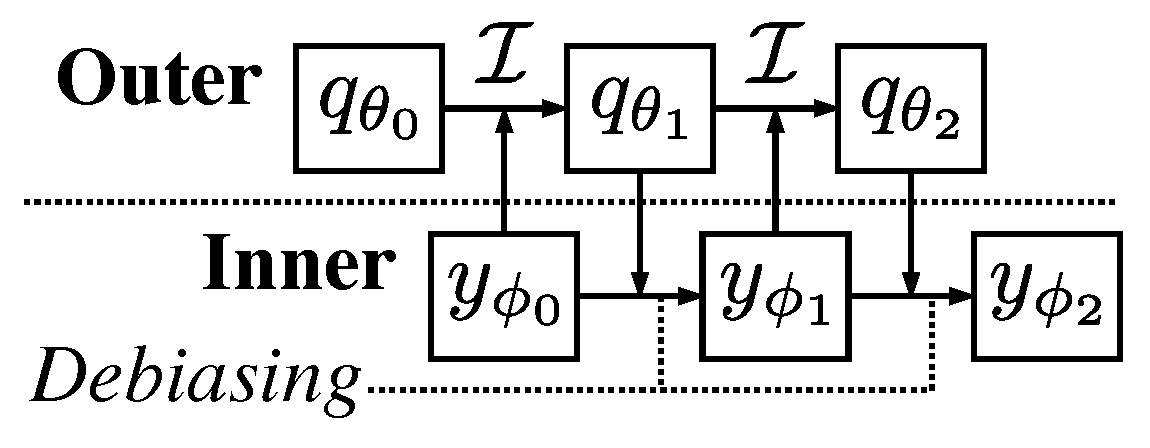
\includegraphics[width=4.2cm]{fig/bi_level.eps}
  \caption{Proposed bi-level learning.}
  \label{fig:bi level}
\end{subfigure}
\caption{
  \emph{Debiasing} is the process of using a propensity model $\propensityName_\propensityParam$ to train a rating model $\ratingName_\ratingParam$ ($\propensityParam_\step$ and $\ratingParam_\step$ are values of model parameters at training step $\step=0,1,2$).
  During debiasing, two-phase learning does not learn the propensity model (pre-trained by a likelihood function $\likelihood{}$), but bi-level learning does (using the rating model's recommendation inaccuracy $\inaccuracy{}$).
%   During \emph{debiasing} (using propensity model $\propensityName_\propensityParam$ to train rating model $\ratingName_\ratingParam$), two-phase learning does not learn the propensity model ($\propensityName_{\propensityParam_2}$ is pre-trained by likelihood function $\likelihood{}$), but bi-level learning does by using the rating model's recommendation inaccuracy $\inaccuracy{}$.
%   $\ratingParam_\step$ and $\propensityParam_\step$ are parameter values of a rating and a propensity model at training step $\step=0$, 1, etc.
}
\end{figure}%
\end{minipage}
\end{figure}

To address the above issues, we propose a bi-level learning approach, which is illustrated in Fig.~\ref{fig:bi level}.
Our main idea is that the best propensity model should minimize the recommendation inaccuracy of the rating model on an unbiased dataset.
Following this idea, we design a nested formulation:
(\myroman{1}) At \textbf{inner} level (see bottom half of Fig.~\ref{fig:bi level}), similar to the two-phase learning, we minimize a propensity-weighted loss to train a rating model.
(\myroman{2}) At \textbf{outer} level (see top half of Fig.~\ref{fig:bi level}), however, we directly minimize the rating model's recommendation inaccuracy on an unbiased dataset to learn a propensity model.
Our approach is named \emph{\underline{l}earning \underline{t}o \underline{d}ebias} (LTD) because it differs from the two-phase learning in that the propensity model is not fixed and is learned during \emph{debiasing} (see bottom half of Fig.~\ref{fig:bi level}).
% We unify the formulations of an inverse-propensity-scoring (IPS) and a doubly-robust (DR) loss, such that LTD is applicable to enhance recent approaches using propensity-weighted losses~\cite{schnabel2016recommendations,wang2019doubly}.
The propensity model learned this way can use all features of observed ratings, e.g., the true rating itself.
These features are often sparse, and thus we propose using a neural architecture for the propensity model to effectively exploit these features.
The neural architecture learns new latent features to enrich the original sparse features, and feeds the enriched features into a stack of hidden layers to estimate propensities.
% employs a stack of hidden layers on top of the enriched features to estimate propensities.
% The neural architecture improves the expressiveness of existing architectures~\cite{ren2018learning,schnabel2016recommendations}.

Given the LTD formulation as bi-level learning, it is challenging to train the propensity model's parameters because propensity-weighted losses often cannot be minimized in closed form.
We tackle this challenge by defining an update function that simulates parameter update of the rating model, and applying back-propagation on this update function to obtain gradients for training the propensity model.
However, unlike prior bi-level learning studies~\cite{franceschi2017forward}, it is also challenging to prevent the training of the rating model from diverging because propensity-weighted losses may produce unstable gradients~\cite{swaminathan2015counterfactual}.
To tackle this challenge, we use the sample variance of estimated propensities per mini-batch to regularize the training of the propensity model, which effectively reduces the variance of propensity estimation.

Our main contributions are summarized as follows.
\begin{itemize}[topsep=0pt,leftmargin=*,noitemsep,wide=0pt]
\item
We propose a bi-level learning approach, learning to debias, for training recommender systems.
It uses a nested formulation to directly model the impact of a propensity model towards the recommendation inaccuracy of a rating model.
% This approach addresses the issue of existing approaches being subject to the error and variance of propensity estimation.
\item
We design a neural architecture for the propensity model by employing a stack of hidden layers on top of learned latent features.
To train the propensity model's parameters, we differentiate an update function that simulates parameter update of the rating model.
We regularize the training of the propensity model with the variance of propensity estimation to obtain stable gradients for training the rating model.
\item
We use four real-world datasets for experiments.
The experiments show that our approach achieves significant improvements (up to a 7.9\% drop in the recommendation inaccuracy) when evaluated on unbiased or biased datasets.
\end{itemize}

\section{Related Work}
Our work is related to prior studies on debiasing problems for recommendation and approaches of bi-level learning.

\subsubsection{Recommendation Debiasing}
Existing studies on recommendation debiasing focus on two tasks: rating prediction and item ranking~\cite{steck2013evaluation}.
The rating prediction task aims to predict the rating that a user may give to an unseen item, whereas the item ranking task aims to provide a user with an item list that maximizes a ranking metric~\cite{steck2010training}.
Both tasks have been widely studied in the past few years~\cite{wang2018confidence}.
In this paper, we solve the rating prediction task.
To solve this task, existing studies often design a certain model architecture (e.g., factorization machine) that computes a real value for each user-item pair~\cite{tay2019holographic}.
Our approach benefits from advances in designing such model architectures, which can be used to implement the underlying rating model~\cite{he2017neural}.

A well-known problem in the rating prediction task is that datasets for training are usually biased~\cite{marlin2007collaborative}.
To handle biased datasets, early studies optimize a joint likelihood of a propensity and a rating model, which requires highly complex inferences~\cite{marlin2009collaborative,hernandez2014probabilistic}.
To avoid such inference complexity, recent studies adopt a two-phase learning approach that first learns a propensity model and then applies propensity weighting techniques to train a rating model~\cite{schnabel2016recommendations,wang2019doubly}.
The main difference between these studies and our work is that our approach allows directly optimizing a propensity model towards the final goal of rating prediction, i.e., minimizing the recommendation inaccuracy of a rating model.

% Such a two-phase learning process is prone to the error and variance of propensity estimation, which is what we aim to address in this paper.
% Specifically, we propose a bi-level learning approach which estimates propensities by directly optimizing the recommendation accuracy.

As for the item ranking task, recent studies show that directly using biased datasets in learning to rank approaches yields sub-optimal results~\cite{ai2018unbiased,joachims2017unbiased}.
These studies on item ranking are largely orthogonal to our work on rating prediction.

\subsubsection{Bi-level Learning}
% which consists of a inner-level and an outer-level learning process
Recently, bi-level learning, which performs outer-level learning subject to the optimality of inner-level learning, has received increasing attention~\cite{maclaurin2015gradient,jenni2018deep}.
Among existing approaches of bi-level learning, the most related one is from Ren et al.~(\citeyear{ren2018learning}), which weights training examples by treating each weight as a parameter to be learned at the outer level.
This approach may generate negative weights, and it resorts to heuristics for adjusting these weights to avoid unstable training behaviors.
In contrast, our approach generates non-negative propensities to weight training ratings by employing a neural architecture.

A widely-recognized challenge in bi-level learning is to compute gradients due to lack of closed form solution to the inner-level learning~\cite{frecon2018bilevel,shaban2019truncated}.
To tackle this challenge, an early approach applies implicit differentiation, and assumes that the optimality to the inner-level learning uniquely exists~\cite{pedregosa2016hyperparameter}.
This assumption often does not hold in practice, and thus this approach may have large errors in gradient computation.
To address this issue, a recent approach computes gradients by differentiating a certain parameter update function for the inner-level learning~\cite{franceschi2018bilevel}.
We further develop this approach by regularizing the training at the outer level with the variance of propensity estimation, which helps stabilize the training at the inner level.


\section{Preliminaries}
Let $\{u_\iUser|\iUser=1,...,\nUser\}$ be users, $\{i_\iItem|\iItem=1,...,\nItem\}$ be items, and $\allPairs=\{(u_\iUser,i_\iItem)|\iUser=1,...,\nUser;\iItem=1,...,\nItem\}$ be all user-item pairs.
Let $\biasedFeatures=\{\feature|\iFeature=1,...,\nFeature\}$ be a feature vector, where element $\feature$ is the $\iFeature$-th feature of user $u$ and item $i$.
Let $\trueRatings=\{\biasedRating|u,i\in\allPairs\}$ be a true rating matrix, where entry $\biasedRating$ is the true rating given by user $u$ to item $i$.
Since users may freely select a fraction of items to rate, we can split all entries of the true rating matrix into observed $\trueRatings^\obsBiasedPairs$ or missing $\trueRatings^\misBiasedPairs$ ratings ($\obsBiasedPairs\cap\misBiasedPairs=\varnothing$ and $\obsBiasedPairs\cup\misBiasedPairs=\allPairs$).
This way, the observed ratings are biased, i.e., the probabilities of observing different ratings are not the same (see Appx.~\ref{app:additional preliminaries} for a more general definition of biasedness)~\cite{marlin2007collaborative}.
Such a probability is usually referred to as the propensity $\propensity=p(\observation=1)$, where $\observation$ is a Bernoulli variable indicating whether the true rating $\biasedRating$ is observed $\observation=1$ or missing $\observation=0$.
% $\observation=\llbracket\biasedRating\in\trueRatings^\obsBiasedPairs\rrbracket$~\footnote{$\llbracket\cdot\rrbracket=1$ if the condition enclosed is true, and $\llbracket\cdot\rrbracket=0$ otherwise.}
Given the biased ratings $\trueRatings^\obsBiasedPairs$, the debiasing problem aims to learn a rating model $\ratingModel\approx\biasedRating$ (with parameters $\ratingParam$) that can accurately predict all true ratings.
In other words, the goal is to minimize the recommendation inaccuracy $\inaccuracy{}$ of a rating model, which can be measured by squaring and averaging all prediction errors $\trueError$ ($u,i\in\allPairs$) of the rating model
\begin{equation*}
\inaccuracy{}
=\frac{1}{\nUser\nItem}
\lrdense{\sum}{u,i\in\allPairs}(\trueError)^2
\defeq\frac{1}{\nUser\nItem}
\lrdense{\sum}{u,i\in\allPairs}(\ratingModel-\biasedRating)^2.
\end{equation*}%

To solve the debiasing problem, recent approaches perform learning in two sequential phases~\cite{schnabel2016recommendations,wang2019doubly}.
(1) The first phase aims to learn a propensity model $\propensityModel\approx\propensity$ (with parameters $\propensityParam$) that can accurately estimate the propensities.
A type of propensity models is a naive Bayes model.
It assumes that the propensity $\propensity=p(\observation=1|\biasedRating=\ratingScale)$ only depends on the true rating, and estimates the propensity by the Bayes' theorem
\begin{equation*}
\propensityModel
=\frac{\nbCondition_{\ratingScale|\obsIndicator}\nbObservation_\obsIndicator}{\nbRating_\ratingScale}
\defeq
\frac{p(\biasedRating=\ratingScale|\observation=1)p(\observation=1)}{p(\biasedRating=\ratingScale)},
\end{equation*}%
where $\propensityParam=\{\nbObservation_\obsIndicator,\nbCondition_{\ratingScale|\obsIndicator},\nbRating_\ratingScale|\ratingScale=1,...,\nScale\}$ are parameters.
To fit the parameters, we may ask users to rate randomly selected items.
This way, the observed ratings $\trueRatings^\obsUnbiasedPairs$ are unbiased, i.e., the propensities of observing different ratings are the same.
Given the biased $\trueRatings^\obsBiasedPairs$ and the unbiased $\trueRatings^\obsUnbiasedPairs$ ratings, the parameters are fitted by maximizing a likelihood function
\begin{equation*}
\max_{\propensityParam}\likelihood{NB}(\propensityParam)
=\lrdense{\prod}{u,i\in\obsBiasedPairs}\nbObservation_\obsIndicator
\lrdense{\prod}{u,i\in\misBiasedPairs}(1-\nbObservation_\obsIndicator)
+\lrdense{\prod}{u,i\in\obsBiasedPairs}\nbCondition_{\biasedRating|\obsIndicator}
+\lrdense{\prod}{u,i\in\obsUnbiasedPairs}\nbRating_{\biasedRating}.
\end{equation*}%
% On the contrary, a logistic regression model assumes that the propensity $\propensity=p(\observation=1|\biasedFeatures)$ depends on the features $\biasedFeatures$, and estimates the propensity by a logistic function
Another type of propensity models is a logistic regression model.
It estimates the propensity by applying a logistic function on the features $\biasedFeatures$ with the true rating excluded
\begin{equation}
\label{eqn:logistic regression model}
\propensityModel
=\sigma(\lgWeight^\transpose\biasedFeatures+\lgBias)
=\frac{\exp(\lgWeight^\transpose\biasedFeatures+\lgBias)}
{\exp(\lgWeight^\transpose\biasedFeatures+\lgBias)+1}.
\end{equation}%
Here, $\propensityParam=\{\lgWeight,\lgBias\}$ are parameters, which are fitted to the biased ratings $\trueRatings^\obsBiasedPairs$ by maximizing another likelihood function
\begin{equation*}
\max_{\propensityParam}\likelihood{LR}(\propensityParam)
=\lrdense{\prod}{u,i\in\obsBiasedPairs}\propensityModel
\lrdense{\prod}{u,i\in\misBiasedPairs}(1-\propensityModel).
\end{equation*}%
% The parameters of the propensity models are learned by maximizing a likelihood function that is not related to the recommendation inaccuracy (see Appx.~\ref{app:additional preliminaries} for details).
(2) Given the propensity model, the second phase aims to train a rating model by minimizing a propensity-weighted loss, e.g., an inverse-propensity-scoring (IPS) or a doubly-robust (DR) loss~\cite{schnabel2016recommendations,wang2019doubly}.
% To this end, Schnabel et al.~(\citeyear{schnabel2016recommendations}) minimize an inverse-propensity-scoring (IPS) loss, whereas Wang et al.~(\citeyear{wang2019doubly}) minimize a doubly-robust (DR) loss.
The DR loss needs an error model $\errorModel\approx\trueError$ (with parameters $\errorParam$) that can accurately impute the prediction errors.

These two-phase learning approaches have an issue that the likelihood function (i.e., the objective for learning the propensity model) is not related to the recommendation inaccuracy.
Thus, maximizing the likelihood function does not necessarily lead to a drop in the recommendation inaccuracy.
Moreover, another issue is that the propensity model is fixed and is not learned during training the rating model.
This way, the error and variance of propensity estimation will propagate into the training at the second phase, which may cause high recommendation inaccuracy~\cite{schnabel2016recommendations}.
% Moreover, it is vulnerable to the error and variance of propensity estimation because fixing the propensity model at the second phase will propagate such error and variance into training the rating model, which may lead to high recommendation inaccuracy.
% and hence cause high recommendation inaccuracy~\cite{schnabel2016recommendations,wang2019doubly}.


\section{Learning to Debias}
To address the issues, we propose \emph{\underline{l}earning \underline{t}o \underline{d}ebias} (LTD), which employs a neural architecture to estimate propensities given sparse features (Sec.~\ref{sec:ltd formulation}).
% First, we formulate LTD as a bi-level learning approach, which employs a neural architecture for propensity estimation (Sec.~\ref{sec:ltd formulation}).
Next, we develop a variance-regularized training algorithm to tackle two challenges in training model parameters within LTD (Sec.~\ref{sec:ltd training}).

\subsection{LTD Formulation and a Neural Architecture}
\label{sec:ltd formulation}
% The key idea of LTD is to nest learning a rating model within learning a propensity model.
% This way, we can improve propensity estimation by propagating back the error of rating prediction on an unbiased dataset.
% Following this idea gives rise to the challenge of capturing the complex dependency of propensities on user and item features, which are often high-dimensional and extremely sparse.
% To address this challenge, we propose a neural architecture that employs a stack of linear layers on top of feature embeddings and interactions to model the dependency in a non-linear way.

We formulate LTD as a bi-level learning approach, which consists of inner-level (\myroman{1}) and outer-level (\myroman{2}) learning.
The inner-level and the outer-level learning require biased $\trueRatings^\obsBiasedPairs$ and unbiased $\trueRatings^\obsUnbiasedPairs$ ratings, respectively.
Typically, the number of the unbiased ratings is much smaller than that of the biased ratings $|\obsUnbiasedPairs|\ll|\obsBiasedPairs|$ because the unbiased ratings are often expensive to obtain in practice~\cite{marlin2007collaborative}.

(\myroman{1}) The inner-level learning, which is equivalent to the second phase of the two-phase learning, aims to train a rating model given a propensity model.
To give a unified treatment of the two-phase learning, we minimize an inner loss $\loss{\innerMark}$ that unifies the formulations of the IPS and the DR loss
\begin{equation}
\label{eqn:inner level learning}
\ratingParam^*(\propensityParam)
=\min_{\ratingParam}\loss{\innerMark}(\ratingParam,\propensityParam)
=\lrdense{\sum}{u,i\in\obsBiasedPairs}\obsLoss_{u,i}(\propensityParam)
+\lrdense{\sum}{u,i\in\misBiasedPairs}\misLoss_{u,i}(\lnot\propensityParam),
\end{equation}%
where $\obsLoss_{u,i}(\propensityParam)$ and $\misLoss_{u,i}(\lnot\propensityParam)$ are losses for the observed $\trueRatings^\obsBiasedPairs$ and the missing $\trueRatings^\misBiasedPairs$ ratings, respectively.
As we will see, $\obsLoss_{u,i}(\propensityParam)$ and $\misLoss_{u,i}(\lnot\propensityParam)$ are denoted this way because the former depends on the propensity model's parameters ($\propensityParam$) but the latter does not ($\lnot\propensityParam$).
We can instantiate the inner loss by IPS as follows.
The IPS loss ignores all missing ratings $\misLoss_{u,i}(\lnot\propensityParam)=0$ ($u,i\in\misBiasedPairs$), and minimizes a square prediction error $\trueLoss$ of the rating model, inversely weighted by an estimated propensity $\propensityModel$, for an observed rating
\begin{equation*}
% \label{eqn:square prediction error}
\obsLoss_{u,i}(\propensityParam)
=\frac{\trueLoss}{\propensityModel}
\defeq\frac{(\ratingModel-\biasedRating)^2}{\propensityModel}
\ (u,i\in\obsBiasedPairs).
\end{equation*}%
Alternatively, we can instantiate the inner loss by DR.
The DR loss treats an imputed error $\errorName_{\errorParam}(\biasedFeatures)$ as the prediction error to train the rating model.
It obtains a ``true rating'' $\imputedRating=\ratingName_{\ratingParam_\step}(\biasedFeatures)+\errorName_{\errorParam_\step}(\biasedFeatures)$ by adding a predicted rating and an imputed error at current training step $\step$.
For a missing rating, it minimizes a square imputed error $\imputedLoss$ between the rating model's next prediction and the ``true rating''
\begin{equation*}
% \label{eqn:square imputed error}
\misLoss_{u,i}(\lnot\propensityParam)
=\imputedLoss
=(\ratingModel-\imputedRating)^2
\ (u,i\in\misBiasedPairs).
\end{equation*}%
Once the true rating is observed, it further adds a correction $\trueLoss-\imputedLoss$ that applies the square prediction error to correct the square imputed error above, and inversely weights this correction by the estimated propensity $\propensityModel$
%in Eqn.~(\ref{eqn:square imputed error})
\begin{equation*}
\obsLoss_{u,i}(\propensityParam)
=\imputedLoss+\frac{\trueLoss-\imputedLoss}{\propensityModel}
\ (u,i\in\obsBiasedPairs).
\end{equation*}%

% The IPS loss ignores missing ratings (Eqn.~\ref{eqn:ips mis}), and uses estimated propensities to inversely weight square prediction errors for observed ratings (Eqn.~\ref{eqn:ips obs}).
% Hence, the inner loss is identical to IPS if the losses are defined by
% \begin{align}
% &\misLoss_{u,i}(\lnot\propensityParam)=0
% \ (u,i\in\misBiasedPairs),
% \label{eqn:ips mis}\\
% &\obsLoss_{u,i}(\propensityParam)=\frac{(\ratingModel-\biasedRating)^2}{\propensityModel}
% \ (u,i\in\obsBiasedPairs).
% \label{eqn:ips obs}
% \end{align}%
% The DR loss treats imputed errors as prediction errors for the missing ratings (Eqn.~\ref{eqn:dr mis}), and applies corrections to imputed errors once the true ratings are observed (Eqn.~\ref{eqn:dr obs}).
% Hence, the inner loss is identical to DR if the losses are defined by
% \begin{align}
% &\misLoss_{u,i}(\lnot\propensityParam)=\imputedLoss
% \ (u,i\in\misBiasedPairs),
% \label{eqn:dr mis}\\
% &\obsLoss_{u,i}(\propensityParam)
% =\frac{\trueLoss-\imputedLoss}{\propensityModel}+\imputedLoss
% \ (u,i\in\obsBiasedPairs),
% \label{eqn:dr obs}
% \end{align}
% where $\trueLoss$ and $\imputedLoss$ are squared losses that use the true rating $\biasedRating$ and the imputed error $\errorModel$ as training signals for the rating model, respectively
% \begin{equation*}
% \begin{aligned}
% \trueLoss&=(\ratingModel-\biasedRating)^2,\\
% \imputedLoss&=(\ratingModel-\errorModel-\stopgrad(\ratingModel))^2.
% \end{aligned}
% \end{equation*}%
% Here, $\stopgrad(\cdot)$ is the operator of stop gradient that sets the gradients of its operand to zero, i.e., $\stopgrad(\ratingModel)=\ratingModel$ and $\nabla_{\ratingParam}\stopgrad(\ratingModel)=0$~\footnote{This operator $\stopgrad$ is available in TensorFlow as \verb~stop\_gradient~.}.
% This operator is used such that minimizing the squared error $\imputedLoss$ will change the predicted rating $\ratingModel$ by the amount of the imputed error.

(\myroman{2}) The outer-level learning aims to learn a propensity model such that the resulting rating model trained by the inner-level learning has low recommendation inaccuracy on an unbiased dataset.
% that minimizes the recommendation inaccuracy of the rating model on an unbiased dataset.
To this end, we minimize an outer loss $\loss{\outerMark}$ that measures how inaccurate the best rating model to the inner loss is at predicting the unbiased ratings $\trueRatings^\obsUnbiasedPairs$
\begin{equation}
\label{eqn:outer level learning}
\propensityParam^*
=\min_{\propensityParam}\loss{\outerMark}(\ratingParam^*(\propensityParam))
=\lrdense{\sum}{u,i\in\obsUnbiasedPairs}
(\ratingName_{\ratingParam^*(\propensityParam)}(\biasedFeatures)-\biasedRating)^2.
\end{equation}%
Since the outer loss relies on the best parameter values $\ratingParam^*(\propensityParam)$ to the inner loss, LTD is considered to have a \emph{nested formulation}: the inner-level learning by Eqn.~(\ref{eqn:inner level learning}) is nested within the outer-level learning by Eqn.~(\ref{eqn:outer level learning}).
Through this nested formulation, LTD directly relates the objective (i.e., the outer loss) for learning the propensity model to the recommendation inaccuracy.
The reason why LTD uses unbiased ratings at the outer level is to be consistent with evaluation procedure: unbiased ratings are often used to unbiasedly evaluate the recommendation inaccuracy~\cite{wang2019doubly}.
% By using the unbiased ratings, the outer loss establishes a direct connection between the propensity model and the recommendation inaccuracy of the rating model.
% Hence, optimizing the outer loss is expected to help the rating model achieve lower recommendation inaccuracy.
% The outer-level learning is based on a basic assumption: the most accurate propensity model should optimize the recommendation inaccuracy on an unbiased dataset consistent with evaluation procedure.%~\footnote{This assumption has been widely adopted, e.g., cross validation assumes that the best hyper-parameters should optimize the performance on a validation set consistent with evaluation procedure.}.
% Compared with the biased set, the unbiased set is expensive to obtain because asking users to rate items that they dislike negatively affects their experiences.

\begin{figure}[t]
\centering
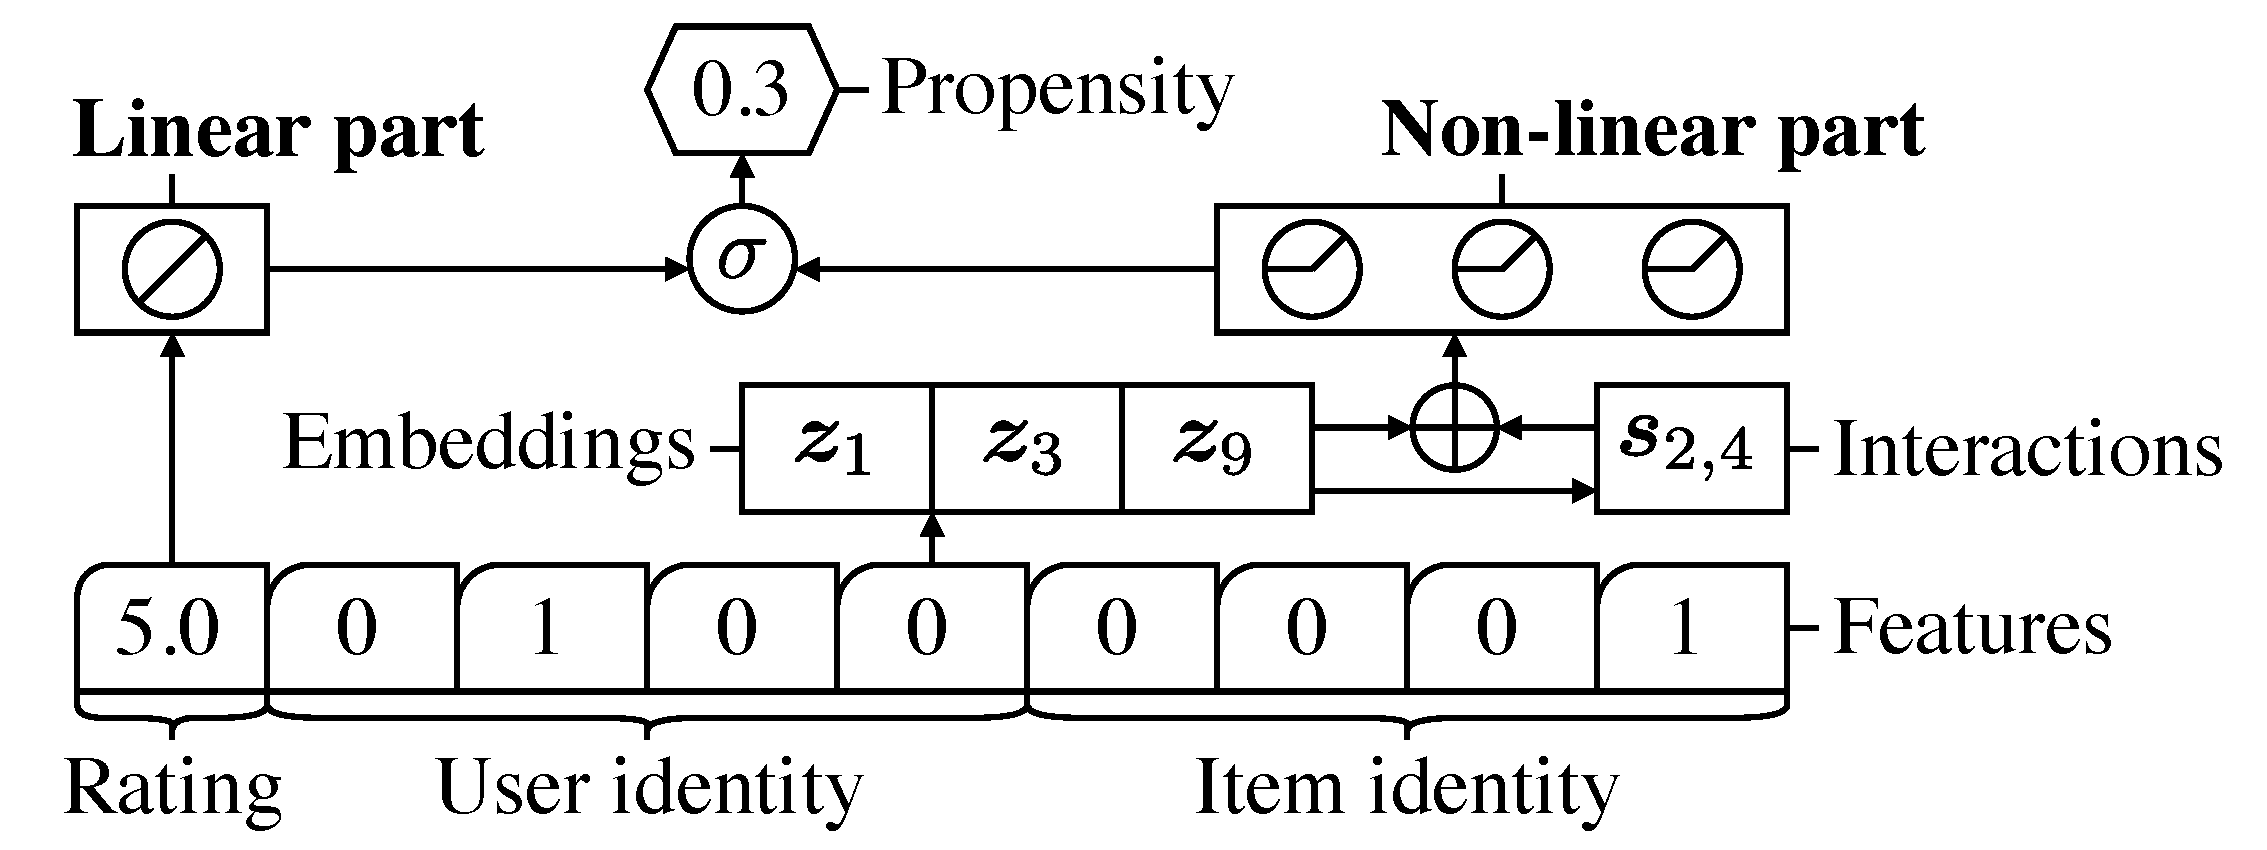
\includegraphics[width=8.4cm]{fig/npm.eps}
\caption{
  Illustration of neural propensity model, which outputs a propensity given sparse features.
  $\npEmbedding_1$, $\npEmbedding_3$, and $\npEmbedding_9$ are embeddings for the 1st, the 3rd, and the 9th feature, respectively.
  $\npSecondOrder_{2,4}$ are second-order feature interactions for the 2nd user and the 4th item.
}
\label{fig:neural propensity model}
\end{figure}%

\subsubsection{Neural Architecture}
An advantage of the LTD formulation is that when learning the propensity model, we only need propensities of the observed ratings $\trueRatings^\obsBiasedPairs$, and do not need those of the missing ratings $\trueRatings^\misBiasedPairs$.
Hence, the propensity model can use extra features that are only available for the observed ratings and are not available for the missing ratings (see Appx.~\ref{app:additional experiments} for all features used).
An example of such a feature is the true rating itself, which is highly correlated with the propensity and thus can be exploited to improve propensity estimation~\cite{marlin2007collaborative}.
% With slight abuse of notation, we still use $\biasedFeatures$ to denote the features used by the propensity model.
To make use of this advantage, we propose a neural architecture as follows.

First, we analyze the issues of existing architectures for the propensity model.
A simple propensity model estimates the propensity $\propensityModel=\sigma(w_{u,i})$ for each user-item pair $u,i\in\obsBiasedPairs$ separately, where $w_{u,i}\in\realNumber$ is a parameter~\cite{ren2018learning}.
This model has two issues:
(1) It can overfit the small set of unbiased ratings as the number of its parameters is equal to that $|\obsBiasedPairs|$ of the biased ratings.
(2) It ignores the features $\biasedFeatures$, which (e.g., the true rating) can be quite predictive in propensity estimation.
The logistic regression model in Eqn.~(\ref{eqn:logistic regression model}) addresses these issues by combining the features linearly.
Due to its linearity, this model may lack the capability to represent the complex dependency of the propensities on the features that are often sparse.

To address the issues, we propose a neural architecture, called a \emph{neural propensity model}~\footnote{Our model differs from that of He and Chua~(\citeyear{he2017neural}) in two aspects:
(1) Besides interactions, we also feed embeddings into hidden layers because interactions are obtained by aggregating embeddings, which may cause information loss.
(2) We add a sigmoid function on top to generate valid probabilities as values of the propensities.}.
As illustrated in Fig.~\ref{fig:neural propensity model}, it augments the logistic regression model (see linear part on the left) by feeding both feature embeddings and interactions into a stack of hidden layers (see non-linear part on the right)
\begin{equation*}
\propensityModel=\sigma(
  \npLinearWeight^\transpose\biasedFeatures+\npLinearBias
  +\npAugmented(\npNonZero\oplus\npSecondOrder_{u,i})
).
\end{equation*}%
Here, $\oplus$ denotes the operator of concatenation for two vectors.
$\npNonZero=\{\npEmbedding_\iFeature|\feature\neq0;\iFeature=1,...,\nFeature\}$ are the concatenated embeddings for all non-zero features of of user $u$ and item $i$, where $\npEmbedding_\iFeature$ is an embedding vector for the $\iFeature$-th feature $\feature$.
% $\npEmbedding_\iFeature\in\realNumber^\nEmbedding$
$\npSecondOrder_{u,i}$ are second-order interactions between features
\begin{equation*}
\npSecondOrder_{u,i}
% =\frac{1}{2}\Bigg(
%   \lrdense{\sum}{\iFeature=1}^{\nFeature}\feature\npEmbedding_\iFeature
% \Bigg)^2
% -\frac{1}{2}\lrdense{\sum}{\iFeature=1}^{\nFeature}(\feature\npEmbedding_\iFeature)^2.
=\sum_{\iFeature=1}^{\nFeature}\sum_{l=\iFeature+1}^{\nFeature}
\feature\npEmbedding_\iFeature\odot\featureMark_{u,i,l}\npEmbedding_l,
\end{equation*}%
where $\odot$ denotes the operator of element-wise product for two vectors.
The feature embeddings and interactions serve as new \emph{latent features} in order to enrich the original sparse features. 
$\npAugmented(\cdot)$ is a stack of $\nLayer$ hidden layers
\begin{equation*}
\npAugmented(\cdot)=\npLastLayer^\transpose\sigma_{\nLayer-1}(
  \npDeepWeight_{\nLayer-1}^\transpose(
    ...\sigma_1(\npDeepWeight_1^\transpose(\cdot)+\npDeepBias_1)...
  )+\npDeepBias_{\nLayer-1}
).
\end{equation*}%
% where $\sigma_\iLayer(\cdot)$ is an activation function for the $\iLayer$-th hidden layer. $\npLastLayer\in\realNumber^{\sLayer_\nLayer}$, $\npDeepWeight_\iLayer\in\realNumber^{\sLayer_{\iLayer}\times\sLayer_{\iLayer+1}}$, and $\npDeepBias_\iLayer\in\realNumber^{\sLayer_\iLayer+1}$ are parameters.
Here, $\sigma_\iLayer(\cdot)$, $\npDeepWeight_\iLayer$, and $\npDeepBias_\iLayer$ are an activation function, a weight matrix, and a bias vector for the $\iLayer$-th layer.
$\npLastLayer$ is a weight vector for the last layer.
To model the dependency underlying the propensities in a non-linear way, we use a non-linear function as the activation function.
All parameters include $\propensityParam=\{\npLinearWeight,\npLinearBias,\npEmbedding_1,...,\npEmbedding_\nFeature,\npDeepWeight_1,\npDeepBias_1,...,\npDeepWeight_{\nLayer-1},\npDeepBias_{\nLayer-1},\npLastLayer\}$.
% The MLP outputs a scalar by using an identity function as the activation function of its last layer.
% To model the dependency in a non-linear way, the MLP use a non-linear function, e.g. a rectified linear unit (ReLU), as the activation function of its other layers.
% By embedding features into a latent space and modeling interactions between features, we can construct new latent features to enrich the original sparse features and thus alleviate the sparsity issue.

\subsection{LTD Training with Variance Regularization}
\label{sec:ltd training}
Next, we detail how to train the parameters $\{\ratingParam,\propensityParam,\errorParam\}$ of LTD.
There are two challenges: 
(1) The outer loss depends on the best rating model which cannot be obtained in closed form.
Thus, the outer loss is not differentiable, making it difficult to train the propensity model's parameters.
(2) The outer loss is orthogonal to the variance of propensity estimation.
This may result in propensities with high variance.
Such propensities, once inversed, can cause the training of the rating model to diverge due to unstable gradients~\cite{swaminathan2015self}.
To tackle these challenges, we propose a variance-regularized training algorithm as follows.

To simplify notation, we define two operators that compute partial gradients w.r.t. parameters $\parameters\in\{\ratingParam,\propensityParam,\errorParam\}$
\begin{equation*}
\nabla_{\parameters_\step}(\cdot)
=\frac{\partial}{\partial\parameters}(\cdot)
\Big|_{\parameters=\parameters_\step},
% \text{ and }
\quad
\nabla_{\parameters_\step}^\transpose(\cdot)
=(\nabla_{\parameters_\step}(\cdot))^\transpose,
% \nabla_{\ratingParam_\step}(\cdot)
% =\frac{\partial}{\partial\ratingParam}(\cdot)
% \Big|_{\ratingParam=\ratingParam_\step},
% \quad
% \nabla_{\ratingParam_\step}^\transpose(\cdot)
% =(\nabla_{\ratingParam_\step}(\cdot))^\transpose,
\end{equation*}%
where $\parameters_\step$ are values of the parameters $\parameters$ at step $\step$ of training.

(\myroman{1}) The inner loss is differentiable w.r.t. the rating model' parameters.
Hence, we can apply vanilla stochastic gradient descent (SGD) or other SGD variants to update the rating model.
We will apply vanilla SGD for illustrative purpose.
% Specifically, at each training step $\step$, given a mini-batch of observed $\obsBiasedPairs_\step\subset\obsBiasedPairs$ and missing $\misBiasedPairs_\step\subset\misBiasedPairs$ ratings, we update the rating model by
% \begin{equation}
% \label{eqn:actual parameter update}
% \ratingParam_{\step+1}
% =\ratingParam_\step-\learningRate
% \nabla_{\ratingParam_\step}\loss{\innerMark}(\ratingParam,\propensityParam_\step).
% \end{equation}

(\myroman{2}) The outer loss is, however, not differentiable. 
We approximate its gradients w.r.t. the propensity model's parameters as follows.
At each training step $\step$, mini-batches of observed $\obsBiasedPairs_\step\subset\obsBiasedPairs$ and missing $\misBiasedPairs_\step\subset\misBiasedPairs$ ratings are sampled.
First, we define an \emph{update function} that simulates mini-batch parameter update of the rating model by vanilla SGD
\begin{align}
&\ratingParam_{\step+1}(\propensityParam_\step)
=\ratingParam_\step-\learningRate\nabla_{\ratingParam_\step}
\loss{\innerMark}(\ratingParam,\propensityParam_\step),\nonumber\\%\label{eqn:dry parameter update}\\%
&=\ratingParam_\step-\learningRate\Bigg(
  \rdense{\sum}{u,i\in\obsBiasedPairs_\step}\nabla_{\ratingParam_\step}
  \obsLoss_{u,i}(\propensityParam_\step)
  +\lrdense{\sum}{u,i\in\misBiasedPairs_\step}\nabla_{\ratingParam_\step}
  \misLoss_{u,i}(\lnot\propensityParam_\step)
\Bigg),\nonumber
\end{align}%
where $\learningRate\in\realNumber^+$ is a learning rate.
This update function models the impact of the propensity model on the training of the rating model, and does not actually update the rating model's parameters.
Then, we approximate the best parameter values in the outer loss with the parameter values $\ratingParam_{\step+1}(\propensityParam_\step)$ from the update function, and differentiate this update function to compute gradients for training the propensity model
% \begin{equation}
% \label{eqn:propensity model training}
% \propensityParam_{\step+1}
% =\propensityParam_\step
% -\learningRate\nabla_{\propensityParam_\step}
% \loss{\outerMark}(\ratingParam_{\step+1}(\propensityParam)).
% \end{equation}%
\begin{align}
&\propensityParam_{\step+1}
=\propensityParam_\step
-\learningRate\nabla_{\propensityParam_\step}
\loss{\outerMark}(\ratingParam_{\step+1}(\propensityParam)),
\label{eqn:propensity model training}\\
&=\propensityParam_\step
-\learningRate\nabla_{\propensityParam_\step}
\lrdense{\sum}{v,j\in\obsUnbiasedPairs_\step}
(\ratingName_{\ratingParam_{\step+1}(\propensityParam)}(\unbiasedFeatures)-\unbiasedRating)^2,
\nonumber\\
% \lossName_{\ratingParam_{\step+1}(\propensityParam)}(\unbiasedFeatures)\nonumber\\
&=\propensityParam_\step
-\learningRate\lrdense{\sum}{v,j\in\obsUnbiasedPairs_\step}
(\nabla_{\propensityParam_\step}\ratingParam_{\step+1}(\propensityParam))
\nabla_{\ratingParam_{\step+1}(\propensityParam_\step)}^\transpose
(\ratingName_{\ratingParam}(\unbiasedFeatures)-\unbiasedRating)^2,
\nonumber\\
% \lossName_\ratingParam(\unbiasedFeatures),\nonumber\\
&=\propensityParam_\step
+\learningRate^2
% \lrdense{\sum}{\substack{u,i\in\obsBiasedPairs_\step\\v,j\in\obsUnbiasedPairs_\step}}(
% \lrdense{\sum}{u,i\in\obsBiasedPairs_\step;v,j\in\obsUnbiasedPairs_\step}
\ldense{\sum}{u,i\in\obsBiasedPairs_\step}
\rdense{\sum}{v,j\in\obsUnbiasedPairs_\step}
(\nabla_{\propensityParam_\step}\nabla_{\ratingParam_\step}\obsLoss_{u,i}(\propensityParam))
\nabla_{\ratingParam_{\step+1}(\propensityParam_\step)}^\transpose
% (\ratingName_{\ratingParam}(\unbiasedFeatures)-\unbiasedRating)^2,\nonumber
\lossName_\ratingParam(\unbiasedFeatures),
\nonumber
\end{align}
where $\obsUnbiasedPairs_\step\subset\obsUnbiasedPairs$ is a mini-batch of unbiased ratings.
The last equation holds because, by definition, the loss $\misLoss_{u,i}(\lnot\propensityParam)$ is constant w.r.t. the propensity model's parameters.
This equation requires the second-order gradients computed as
\begin{equation*}
\thinmuskip=1.5mu
\medmuskip=2.0mu
\thickmuskip=2.5mu
\begin{aligned}
\nabla_{\propensityParam_\step}\nabla_{\ratingParam_\step}
\obsLoss_{u,i}(\propensityParam)
&=-\frac{
  \nabla_{\propensityParam_\step}\propensityModel
  \nabla_{\ratingParam_\step}^\transpose(\ratingModel-\biasedRating)^2
}{\propensityName_{\propensityParam_\step}(\biasedFeatures)^2},\\
\nabla_{\propensityParam_\step}\nabla_{\ratingParam_\step}
\obsLoss_{u,i}(\propensityParam)
&=-\frac{
  \nabla_{\propensityParam_\step}\propensityModel
  \nabla_{\ratingParam_\step}^\transpose(\trueLoss-\imputedLoss)
}{\propensityName_{\propensityParam_\step}(\biasedFeatures)^2},
\end{aligned}
\end{equation*}%
when using the IPS and the DR loss, respectively.
% \begin{equation*}
% \end{equation*}%
% when using the DR loss at the inner level.

\begin{algorithm}[tbp]
\small
\caption{\small \textalg{Vrt}: Variance-Regularized Training}
\label{alg:vrt}
\KwIn{$\nStep,\trueRatings^\obsBiasedPairs,\trueRatings^\obsUnbiasedPairs,\ratingParam_0,\propensityParam_0,\errorParam_0$}
\For{$\step=0,...,\nStep-1$}{
  Sample mini-batches $\obsBiasedPairs_\step\subset\obsBiasedPairs$ ($\misBiasedPairs_\step\subset\misBiasedPairs$) and $\obsUnbiasedPairs_\step\subset\obsUnbiasedPairs$\label{alg:sample mini batches}\\
  Compute the inner loss $\loss{\innerMark}(\ratingParam_\step,\propensityParam_\step)$ on $\obsBiasedPairs_\step$ (and $\misBiasedPairs_\step$)\label{alg:parameter update start}\\
%   Compute gradients $\nabla_{\ratingParam_\step}\loss{\innerMark}(\ratingParam,\propensityParam_\step)$\\
  Run update function $\ratingParam_{\step+1}(\propensityParam_\step)\leftarrow\ratingParam_\step-\learningRate\nabla_{\ratingParam_\step}\loss{\innerMark}(\ratingParam,\propensityParam_\step)$\label{alg:parameter update stop}\\
  Compute the RO loss $\loss{\rOuterMark}(\ratingParam_{\step+1}(\propensityParam_\step))$ on $\obsUnbiasedPairs_\step$ and $\obsBiasedPairs_\step$\label{alg:update propensity start}\\
%   Compute gradients $\nabla_{\propensityParam_\step}\loss{\rOuterMark}(\ratingParam_{\step+1}(\propensityParam))$\\
  Update parameters $\propensityParam_{\step+1}\leftarrow\propensityParam_\step-\learningRate\nabla_{\propensityParam_\step}\loss{\rOuterMark}(\ratingParam_{\step+1}(\propensityParam))$\label{alg:update propensity stop}\\
  Compute the inner loss $\loss{\innerMark}(\ratingParam_\step,\propensityParam_{\step+1})$ on $\obsBiasedPairs_\step$ (and $\misBiasedPairs_\step$)\label{alg:update rating start}\\
%   Compute gradients $\nabla_{\ratingParam_\step}\loss{\innerMark}(\ratingParam,\propensityParam_{\step+1})$\\
  Update parameters $\ratingParam_{\step+1}\leftarrow\ratingParam_\step-\learningRate\nabla_{\ratingParam_\step}\loss{\innerMark}(\ratingParam,\propensityParam_{\step+1})$\label{alg:update rating stop}\\
}
\KwOut{$\ratingParam_\nStep,\propensityParam_\nStep$}
\end{algorithm}


\begin{figure}[t]
\centering
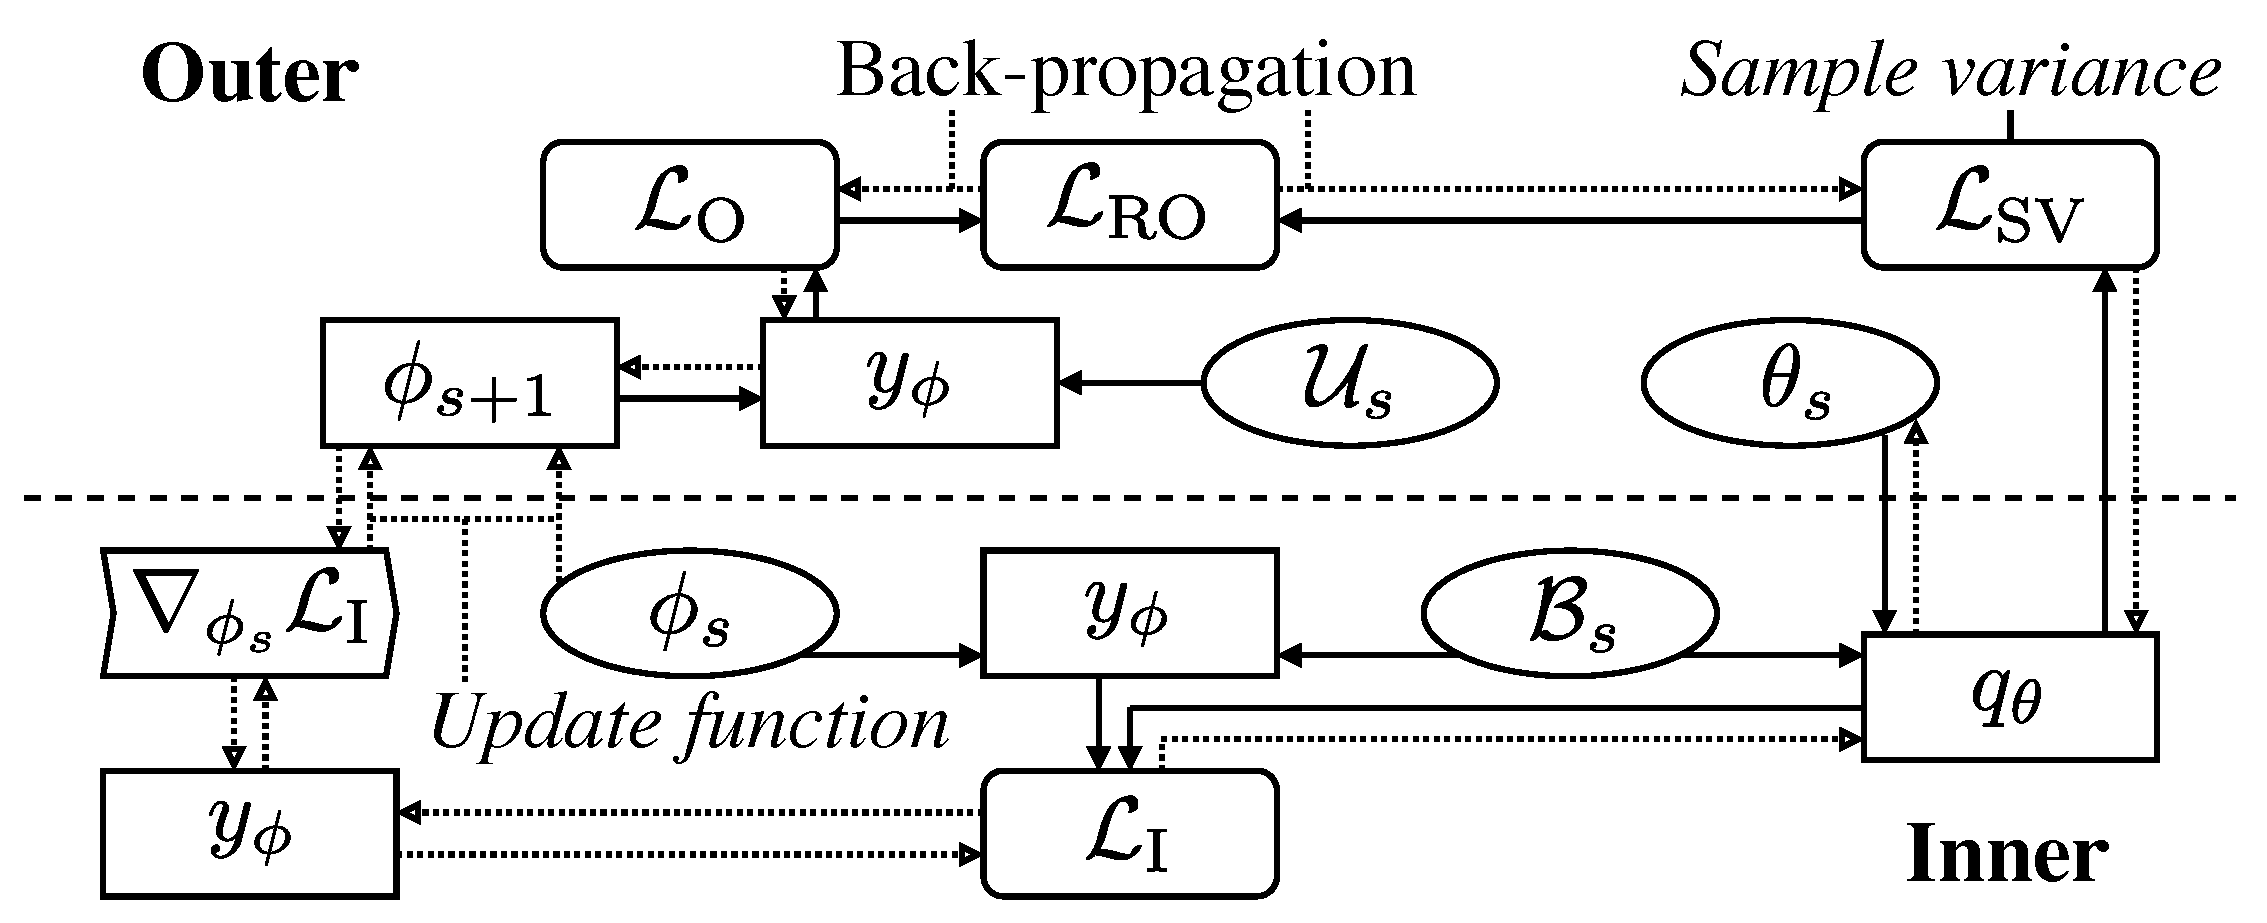
\includegraphics[width=8.4cm]{fig/ltd.eps}
\caption{
  Computational graph of variance-regularized training at step $\step$.
  It starts at eclipses, and applies back-propagation via an \emph{update function} or \emph{sample variance} to train a propensity model $\propensityName_\propensityParam$.
  Solid and dotted lines are forward and backward passes, respectively.
}
\label{fig:computational graph}
\end{figure}%

\subsubsection{Variance Regularization}
We observe that the propensity model trained using the above algorithm in Eqn.~(\ref{eqn:propensity model training}) often has increasing variance in propensity estimation (see Fig.~\ref{fig:variance epoch} for empirical evidence).
Such estimation variance may cause the training of the rating model unstable because a portion of biased ratings may receive low propensities and thus dominate the inner loss.
To reduce the variance of propensity estimation, we propose a regularized-outer (RO) loss that regularizes the outer loss with the sample variance of estimated propensities for the mini-batch $\obsBiasedPairs_\step$ of biased ratings
\begin{equation*}
\loss{\rOuterMark}(\ratingParam_{\step+1}(\propensityParam_\step))
=\loss{\outerMark}(\ratingParam_{\step+1}(\propensityParam_\step))
+\regularization\loss{\varianceMark}(\propensityParam_\step).
\end{equation*}%
Here, $\regularization\in\realNumber^+$ is a regularization hyper-parameter and
\begin{equation*}
\loss{\varianceMark}(\propensityParam_\step)
% =\lrdense{\sum}{u,i\in\obsBiasedPairs_\step}
% \propensityName_{\propensityParam_\step}(\biasedFeatures)^2
% -\frac{1}{|\obsBiasedPairs_\step|}\Bigg(
%   \rdense{\sum}{u,i\in\obsBiasedPairs_\step}
%   \propensityName_{\propensityParam_\step}(\biasedFeatures)
% \Bigg)^2
=\frac{1}{|\obsBiasedPairs_\step|-1}
\rdense{\sum}{u,i\in\obsBiasedPairs_\step}\Bigg(
  \propensityName_{\propensityParam_\step}(\biasedFeatures)
  -\lrdense{\sum}{v,j\in\obsBiasedPairs_\step}
  \frac{\propensityName_{\propensityParam_\step}(\unbiasedFeatures)}{|\obsBiasedPairs_\step|}
\Bigg)^2
\end{equation*}%
is the \emph{sample variance}.
Since the sample variance is differentiable w.r.t. the propensity model's parameters, we can straightforwardly compute the gradients of the RO loss as
\begin{equation*}
\nabla_{\propensityParam_\step}
\loss{\rOuterMark}(\ratingParam_{\step+1}(\propensityParam))
=\nabla_{\propensityParam_\step}
\loss{\outerMark}(\ratingParam_{\step+1}(\propensityParam))
+\regularization\nabla_{\propensityParam_\step}
\loss{\varianceMark}(\propensityParam).
\end{equation*}%
% where the gradients of the sample variance are
% \begin{equation*}
% \begin{aligned}
% \nabla_{\propensityParam_\step}
% \loss{\varianceMark}(\propensityParam_\step)
% &=2\lrdense{\sum}{u,i\in\obsBiasedPairs_\step}
% \propensityName_{\propensityParam_\step}(\biasedFeatures)
% \nabla_{\propensityParam_\step}\propensityModel\\
% &-\frac{2}{|\obsBiasedPairs_\step|}
% \rdense{\sum}{u,i\in\obsBiasedPairs_\step}
% \propensityName_{\propensityParam_\step}(\biasedFeatures)
% \lrdense{\sum}{u,i\in\obsBiasedPairs_\step}
% \nabla_{\propensityParam_\step}\propensityModel.
% \end{aligned}
% \end{equation*}%

%~\footnote{Here, we use automatic differentiation, available in scientific libraries like TensorFlow~\cite{abadi2016tensorflow}, to compute gradients.}.
We show the above algorithm of training the rating and the propensity model with variance regularization in Alg.~\ref{alg:vrt} (the IPS loss ignores missing ratings shown in parentheses).
% At each training step, we first sample mini-batches of training ratings (line~\ref{alg:sample mini batches}).
% Then, we update the propensity model by applying back-propagation on the unrolled training (line~\ref{alg:parameter update start}-\ref{alg:update propensity stop}).
% Next, we use the updated propensity model to perform the actual update of the rating model (line~\ref{alg:update rating start}-\ref{alg:update rating stop}).
% Then, we update the propensity model's parameters along the gradients of the RO loss (line~\ref{alg:parameter update start}-\ref{alg:update propensity stop}), and use the updated propensity model to update the rating model's parameters (line~\ref{alg:update rating start}-\ref{alg:update rating stop}).
% At each training step $\step$, we first sample mini-batches of biased and unbiased ratings (line~\ref{alg:sample mini batches}).
% Then, we update the parameters of the propensity (line~\ref{alg:parameter update start}-\ref{alg:update propensity stop}) and the rating model (line~\ref{alg:update rating start}-\ref{alg:update rating stop}).
For each training step, after sampling mini-batches of biased and unbiased ratings (line~\ref{alg:sample mini batches}), we update the parameters of the propensity (line~\ref{alg:parameter update start}-\ref{alg:update propensity stop}) and the rating (line~\ref{alg:update rating start}-\ref{alg:update rating stop}) model.
We further show the computation involved in a training step by a computational graph in Fig.~\ref{fig:computational graph}.
We first compute losses (see solid lines in Fig.~\ref{fig:computational graph}) and then compute gradients (see dotted lines in Fig.~\ref{fig:computational graph}) for parameter update by applying back-propagation.
We can directly apply Alg.~\ref{alg:vrt} if using the IPS loss, but need to train an extra error model if using the DR loss.
Following Wang et al.~(\citeyear{wang2019doubly}), we train the error model by minimizing an error-imputation (EI) loss that computes a weighted average of square errors between the imputed and the prediction errors given the biased ratings $\trueRatings^\obsBiasedPairs$
\begin{equation*}
% \label{eqn:imputation learning loss}
\min_{\errorParam}\loss{EI}(\errorParam)
=\lrdense{\sum}{u,i\in\obsBiasedPairs}
\frac{(\errorModel-\trueError)^2}{\propensityModel}.
\end{equation*}%
We show the complete algorithm when using the DR loss in Alg.~\ref{alg:drvrt}.
We alternate between training the error and the rating (by Alg.~\ref{alg:vrt}) model until a stopping criteria is satisfied.

\begin{algorithm}[tbp]
\small
\caption{\small Doubly-Robust Variance-Regularized Training}
\label{alg:drvrt}
\KwIn{$\nEpoch,\nStep,\trueRatings^\obsBiasedPairs,\errorParam^0_0,\trueRatings^\obsUnbiasedPairs,\ratingParam_0,\propensityParam_0$}
\For{$\epoch=0,...,\nEpoch-1$}{
  \For{$\step=0,...,\nStep-1$}{
    Sample a mini-batch $\obsBiasedPairs_{\epoch}^{\step}\subset\obsBiasedPairs$\\
    Compute the EI loss $\loss{EI}(\errorParam_{\epoch}^{\step})$ on $\obsBiasedPairs_{\epoch}^{\step}$ \\
    Update parameters $\errorParam_{\epoch}^{\step+1}\leftarrow\errorParam_{\epoch}^{\step}-\learningRate\nabla_{\errorParam_{\epoch}^{\step}}\loss{EI}(\errorParam)$\\
  }
  Call Alg.~\ref{alg:vrt} $\ratingParam_{\epoch+1},\propensityParam_{\epoch+1}\leftarrow\text{\textalg{Vrt}}(\nStep,\trueRatings^\obsBiasedPairs,\trueRatings^\obsUnbiasedPairs,\ratingParam_{\epoch},\propensityParam_{\epoch},\errorParam_{\epoch}^{\nStep})$\\
  Copy parameter values $\errorParam_{\epoch+1}^{0}\leftarrow\errorParam_{\epoch}^{\nStep}$\\
}
\KwOut{$\ratingParam_{\nEpoch},\propensityParam_{\nEpoch},\errorParam_{\nEpoch}^{0}$}
\end{algorithm}


\section{Experiments}
% , after describing our experimental datasets and settings, 
We conduct the following experiments to empirically study the proposed LTD.
First, we compare LTD against the state-of-the-art approaches to the debiasing problem.
Second, we implement the propensity model by different architectures and explore effects of the variance regularization to analyze the main components of LTD.
Third, we inspect estimated propensities from the propensity model to explore how LTD contributes to the training of the rating model by propensity weighting.
Last, we vary the number of the unbiased ratings required by LTD to study the trade-off between smaller unbiased datasets and lower recommendation inaccuracy.

\subsubsection{Datasets}
To our knowledge, only two real-world datasets that contain biased and unbiased ratings are available:
(1) \textsc{Music} has 311,704 biased and 54,000 unbiased ratings by 15,400 users to 1,000 songs~\cite{marlin2007collaborative}.
(2) \textsc{Coat} has 6,960 biased and 4,640 unbiased ratings by 290 users to 300 coats, where covariates (e.g., user gender and coat color) are available~\cite{schnabel2016recommendations}.
To show the scalability of LTD, we use two larger real-world datasets that contain only biased ratings:
(1) \textsc{Book} has 1,273,679 biased ratings by 19,804 users to 22,086 books~\cite{sun2017exploiting}.
Since it is difficult to evaluate collaborative filtering approaches on highly sparse datasets, we ensure that each user or each item has at least 25 ratings.
(2) \textsc{Movie} has 1,000,209 biased ratings by 6,040 users to 3,706 movies, where covariates (e.g., user age and movie genre) are available~\cite{dong2017hybrid}. % 

\subsubsection{Settings}
Approaches that explicitly handle biased datasets and those that do not are called \emph{debiasing} and \emph{traditional} approaches, respectively.
We compare with two traditional approaches: (1) Matrix factorization (\textbf{MF}) using identities of users and items as features~\cite{koren2009matrix}. (2) Neural factorization (\textbf{NF}) using identities and covariates (if available) of users and items as features~\cite{he2017neural}.
We also compare with the following debiasing approaches: (1) \textbf{CPT-V}~\cite{marlin2009collaborative}. (2) \textbf{PMF-NMAR}~\cite{hernandez2014probabilistic}. (3) \textbf{(MF/NF)-IPS} using MF or NF as the rating model~\cite{schnabel2016recommendations}. (4) \textbf{(MF/NF)-DR} using MF or NF as the rating and the error model~\cite{wang2019doubly}.
We use \textbf{(MF/NF)-(IPS/DR)-LTD} to denote our approaches instantiating the inner-level learning by (MF/NF)-(IPS/DR).

To unbiasedly evaluate an approach's capability to handle biased datasets, we treat the biased and the unbiased ratings on \textsc{Music} and \textsc{Coat} as a training and a testing set~\cite{schnabel2016recommendations}.
Since \textsc{Movie} and \textsc{Book} do not have unbiased ratings, we randomly split the biased ratings into a training (90\%) and a testing (10\%) set (the results by a time split are similar and thus omitted)~\cite{li2017ermma}.
We refer to the unbiased ratings required by LTD as the \emph{validation set}.
Following Wang et al.~(\citeyear{wang2019doubly}), we set aside 5\% of the testing set as the validation set.
% Recall that LTD requires the small set in Eqn.~\ref{eqn:outer level learning} to be consistent with the evaluation procedure, we set aside 5\% of the testing set to construct this small set, which we refer to as the \emph{validation set}.
To ensure that LTD does not use more observed ratings than the other approaches, we add this validation set into the training set.
We evaluate an approach by averaging its mean absolute error (MAE) and its mean square error (MSE) on the testing set over 10 different runs.
Due to space limit, we defer the results by MAE, similar to those by MSE, to Appx.~\ref{app:additional experiments}.
We search the same hyper-parameter within the same range across all approaches.
Since \textsc{Music} and \textsc{Book} have neither user nor item covariates, (MF/NF)-(IPS/DR) use the validation set to fit a naive Bayes model.
See Appx.~\ref{app:additional experiments} for more details on our settings.

\subsubsection{Overall Results}
\begin{table}[tbp]
\small
\centering
% \setlength\tabcolsep{6.0pt}
\caption{Average MSE of all approaches over 10 different runs.}
\label{tab:mse overall results}
\begin{threeparttable}
\begin{tabular}{l|cc||cc}
\toprule
& \multicolumn{2}{c||}{Unbiased testing set} & \multicolumn{2}{c}{Biased testing set} \\
\cmidrule(rl){2-5}
Approach & \textsc{Music} & \textsc{Coat} & \textsc{Book} & \textsc{Movie} \\
\midrule
MF & 1.951 & 1.349 & 0.719 & 0.695 \\
NF & 1.586 & 1.299 & 0.656 & 0.657 \\
\midrule
CPT-V & 1.181 & 1.512 & 0.968 & 1.069 \\
PMF-NMAR & 2.243 & 1.279 & 0.714 & 0.691 \\
MF-IPS & 1.069 & 1.179 & 0.730 & 0.708 \\
NF-IPS & 1.047 & 1.137 & 0.672 & 0.662 \\
MF-DR & 1.037 & 1.058 & 0.697 & 0.680 \\
NF-DR & 1.024 & 1.033 & 0.637 & 0.636 \\
\midrule
MF-IPS-LTD & 1.009 & 1.062 & 0.682 & 0.661 \\
NF-IPS-LTD & 0.992 & 1.041 & 0.634 & 0.629 \\
MF-DR-LTD & 0.982 & 0.982 & 0.654 & 0.651 \\
NF-DR-LTD & \textbf{0.977} & \textbf{0.973} & \textbf{0.598} & \textbf{0.619} \\
\bottomrule
\end{tabular}
\begin{tablenotes}[flushleft]
\footnotesize
\item[*] The bottom four rows show the proposed approaches.
\end{tablenotes}
\end{threeparttable}
\end{table}

We show the result by MSE on \textsc{Music} and \textsc{Coat} in the left half of Table~\ref{tab:mse overall results}, where the testing set is unbiased.
We can see that the proposed LTD significantly improves its corresponding two-phase learning approach.
For example, MF-IPS-LTD (1.062) outperforms MF-IPS (1.179) by 9.9\% on \textsc{Coat}.
We also find that NF-DR-LTD performs the best on both datasets, e.g., NF-DR-LTD achieves the smallest MSE (0.977) on \textsc{Music}.
By comparing (MF/NF)-(IPS/DR)-LTD, we can see that LTD benefits from:
(1) Advanced model architecture: NF enhances the expressiveness of MF by modeling non-linear and high-order interactions between features.
(2) Improved inner loss: the DR loss addresses the variance issue of the IPS loss by jointly training the rating and the error model.
In general, the debiasing approaches outperform the traditional ones by explicitly modeling the biasedness in rating observation.
However, the debiasing approaches, CPT-V and PMF-NMAR, perform worst on \textsc{Coat} and \textsc{Music}, respectively.
These two debiasing approaches are probably not properly fit because of making strong generative assumptions and requiring highly complex inferences.
Unlike CPT-V and PMF-NMAR, our approaches neither make generative assumptions nor require complex inferences, which leads to consistent improvements across the datasets.

We show the result by MSE on \textsc{Book} and \textsc{Movie} in the right half of Table~\ref{tab:mse overall results}, where the testing set is biased.
We can see that the debiasing approaches have no clear advantages over the traditional ones.
For example, MF-IPS (0.708) performs even worse than MF (0.695) on \textsc{Movie}.
This is because evaluation on biased datasets is biased, and favors the traditional approaches that assume uniform propensities.
We also find that LTD achieves significant improvements over its traditional and its debiasing counterpart.
For example, NF-DR-LTD (0.598) outperforms NF (0.656) by 8.8\% and outperforms NF-DR (0.637) by 6.1\% on \textsc{Book}.
The reason for such improvements is that unlike the traditional or the debiasing approaches, LTD does not assume uniform or non-uniform propensities.
Instead, LTD assumes that we have a validation set to resolve the distribution mismatch between the training and the testing set.
This makes LTD achieve consistent improvements irrespective of using biased or unbiased datasets for evaluation.
Since NF-DR-LTD performs the best on all four datasets, we will focus on its results in the following.
We observe that the the results of other LTD approaches are similar to those of NF-DR-LTD.

\subsubsection{Ablation Studies}
To study the preferred architecture for propensity estimation, we implement the propensity model of NF-DR-LTD by a simple propensity (SP), a logistic regression (LR), or a neural propensity (NP) model.
We use NP-(1/2/3) to denote a NP model with one, two, or three hidden layers, respectively.
We show the result by MSE on the four datasets in Table~\ref{tab:mse ablation studies}.
We can see that using the NP model with two hidden layers performs the best.
Using more hidden layers does not further reduce the MSE largely because the validation set is too small to learn the extra parameters.
Consistent with our analyses in Sec.~\ref{sec:ltd formulation}, using the SP model performs the worst, especially on \textsc{Book} and \textsc{Movie} with a large training set.
The NP model is preferred over the LR model due to its ability to learn new latent features and capture non-linear dependencies.
We observe that feeding only feature interactions into the hidden layers of the NP model leads to a slightly higher MSE (up to a 1.6\% increase).

We also study how the regularization hyper-parameter affects the inaccuracy of LTD.
We plot the result by MSE on \textsc{Music} in Fig.~\ref{fig:mse var reg}.
We find that the variance regularization is indeed beneficial and the best hyper-parameter $\regularization$ is near~1, e.g., MF-IPS-LTD with $\regularization=1$ (1.009) outperforms that with $\regularization=0$ (1.026) by 1.7\%.
% We also find that LTD achieves the smallest MSE when $\regularization$ is around 1.
We further compute the sample variance of estimated propensities on the testing set.
We show the result during training NF-DR-LTD on \textsc{Music} in Fig.~\ref{fig:variance epoch}.
We can see that the sample variance on the testing set keeps growing when $\regularization=0$, but drops after a few epochs when $\regularization\geq1$.
This indicates that minimizing the sample variance on the training set generalizes well to the testing set.

\begin{table}[tbp]
\small
\centering
\caption{Average MSE of NF-DR-LTD over 10 different runs.}
\label{tab:mse ablation studies}
\begin{tabular}{l|l|cc||cc}
\toprule
% \multicolumn{2}{c|}{} & \multicolumn{2}{c||}{Unbiased testing set} & \multicolumn{2}{c}{Biased testing set} \\
% \cmidrule(rl){3-6}
\multicolumn{2}{c|}{Propensity model} & \textsc{Music} & \textsc{Coat} & \textsc{Book} & \textsc{Movie} \\
\midrule
\multirow{2}{*}{Existing} & SP & 1.044 & 1.028 & 0.727 & 0.699 \\
& LR & 1.003 & 1.006 & 0.668 & 0.655 \\
\midrule
\multirow{3}{*}{Proposed} & NP-1 & 0.988 & 0.981 & 0.636 & 0.633 \\
& NP-2 & \textbf{0.977} & \textbf{0.973} & \textbf{0.598} & \textbf{0.619} \\
& NP-3 & 0.996 & 0.990 & 0.652 & 0.647 \\
\bottomrule
\end{tabular}
\end{table}

\subsubsection{Propensity Weighting}
To explore how LTD contributes to the training by propensity weighting, we average estimated propensities from the neural propensity model over different rating values (e.g., 1-5) on the training set.
We show the result when we complete training NF-DR-LTD on \textsc{Music} in Fig.~\ref{fig:propensity rating}.
We can see that on average larger ratings do have larger propensities, which is consistent with the findings by prior studies~\cite{marlin2007collaborative}.
We further study how such result is achieved by computing the mean propensity over different rating values during training.
We show the result of training NF-DR-LTD on \textsc{Music} in Fig.~\ref{fig:propensity epoch}.
We can see that the larger a rating value is, the slower its mean propensity decreases.
% the mean propensity of large ratings decreases slower than that of small ratings.
These results indicate that by learning from the validation set, LTD inversely weights larger ratings by larger propensities to make the training set less biased.

\subsubsection{Validation Set Size}
\begin{figure}[!t]
\hspace*{-0.44cm}
\begin{minipage}[t]{1.090\linewidth}
\centering
\begin{figure}[H]
\centering
\begin{subfigure}{0.495\textwidth}
  \centering
  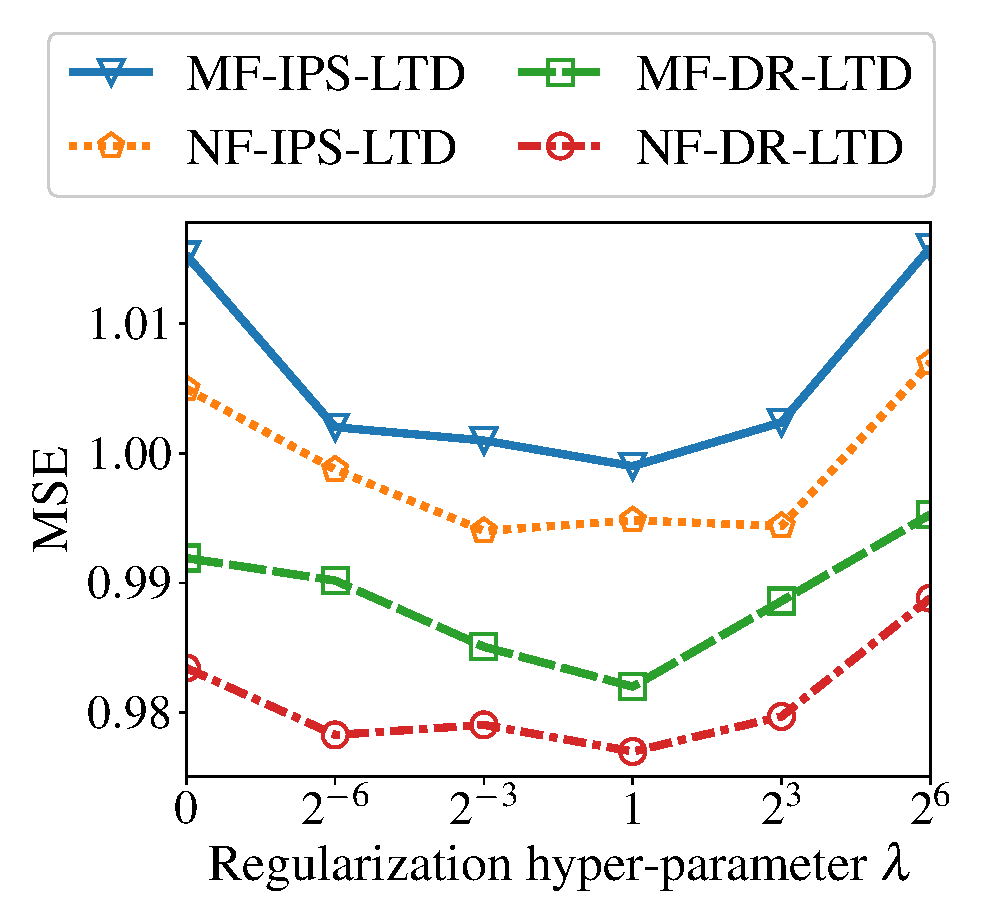
\includegraphics[height=3.76cm]{fig/mse_var_reg.eps}
  \caption{MSE of our approaches.}
  \label{fig:mse var reg}
\end{subfigure}
\hfill % \hspace{-0.45cm}
\begin{subfigure}{0.495\textwidth}
  \centering
  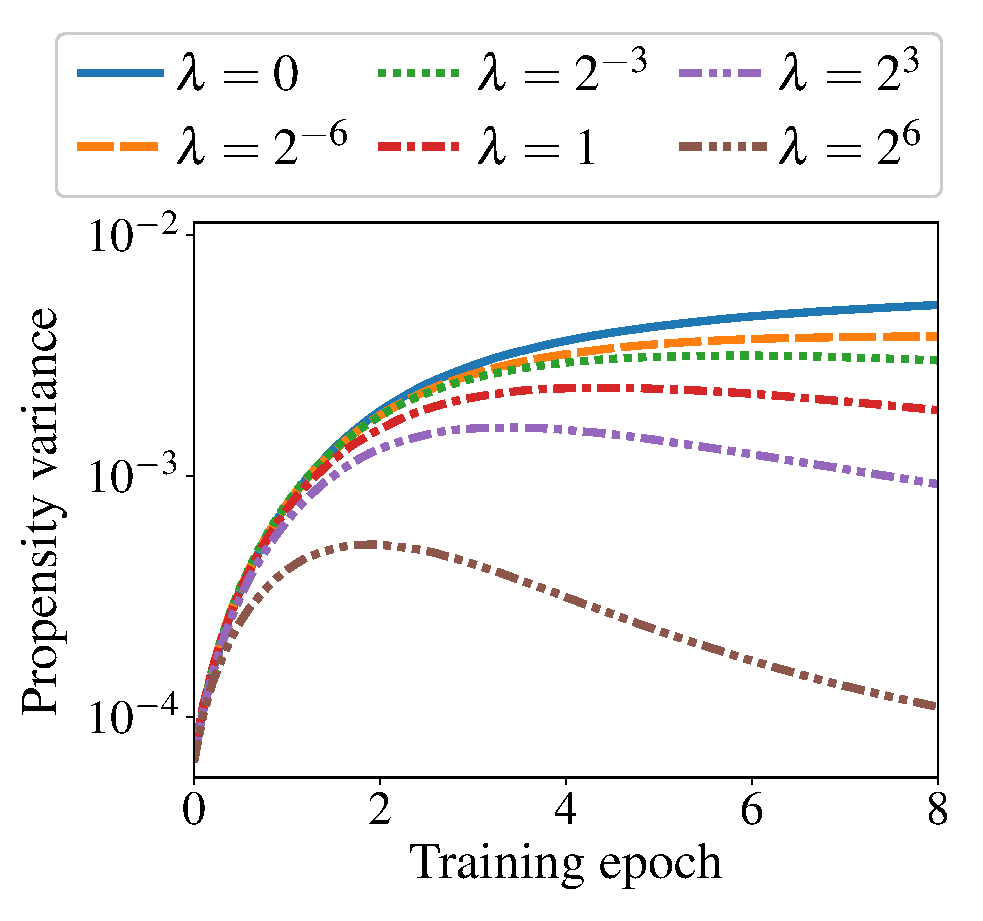
\includegraphics[height=3.76cm]{fig/variance_epoch.eps}
  \caption{Training NF-DR-LTD.}
  \label{fig:variance epoch}
\end{subfigure}
\caption{Effects of the variance regularization on \textsc{Music}.}
\end{figure}%
\end{minipage}
\hspace*{-0.44cm}
\begin{minipage}[t]{1.090\linewidth}
\centering
\begin{figure}[H]
\centering
\begin{subfigure}{0.495\textwidth}
  \centering
  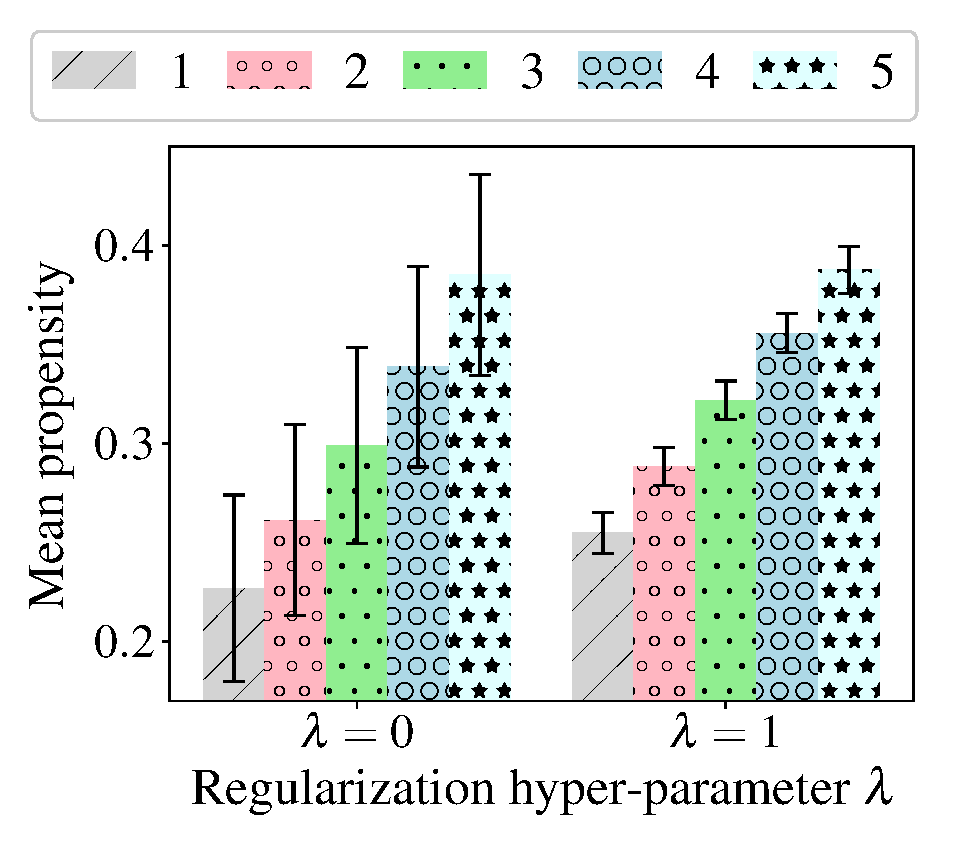
\includegraphics[height=3.46cm]{fig/propensity_rating.eps}
  \caption{Bars show standard deviation.}
  \label{fig:propensity rating}
\end{subfigure}
\hfill % \hspace{-0.45cm}
\begin{subfigure}{0.495\textwidth}
  \centering
  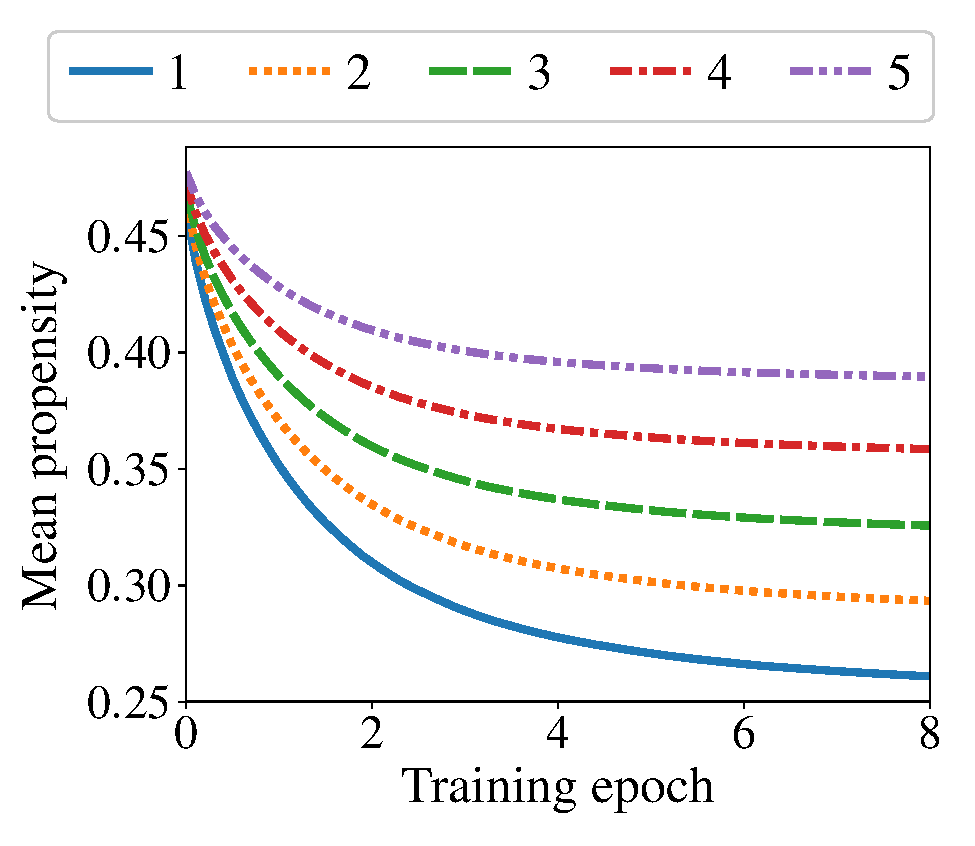
\includegraphics[height=3.46cm]{fig/propensity_epoch.eps}
  \caption{Hyper-parameter $\regularization=1$.}
  \label{fig:propensity epoch}
\end{subfigure}
\caption{Mean propensity by NF-DR-LTD over rating value 1-5 on \textsc{Music}.}
\end{figure}%
\end{minipage}
\hspace*{-0.44cm}
\begin{minipage}[t]{1.090\linewidth}
\centering
\begin{figure}[H]
\centering
\begin{subfigure}{0.495\textwidth}
  \centering
  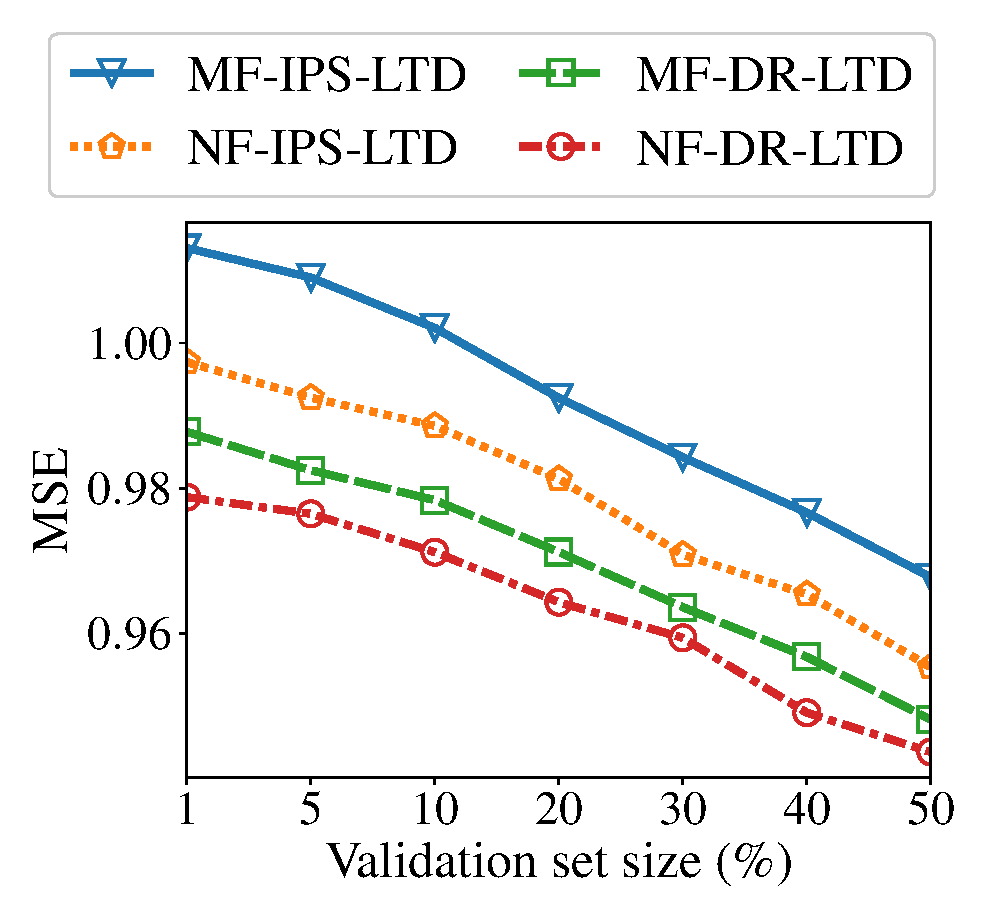
\includegraphics[height=3.88cm]{fig/mse_unbiased_size.eps}
  \caption{MSE of our approaches.}
  \label{fig:validation set inaccuracy}
\end{subfigure}
\hfill % \hspace{-0.45cm}
\begin{subfigure}{0.495\textwidth}
  \centering
  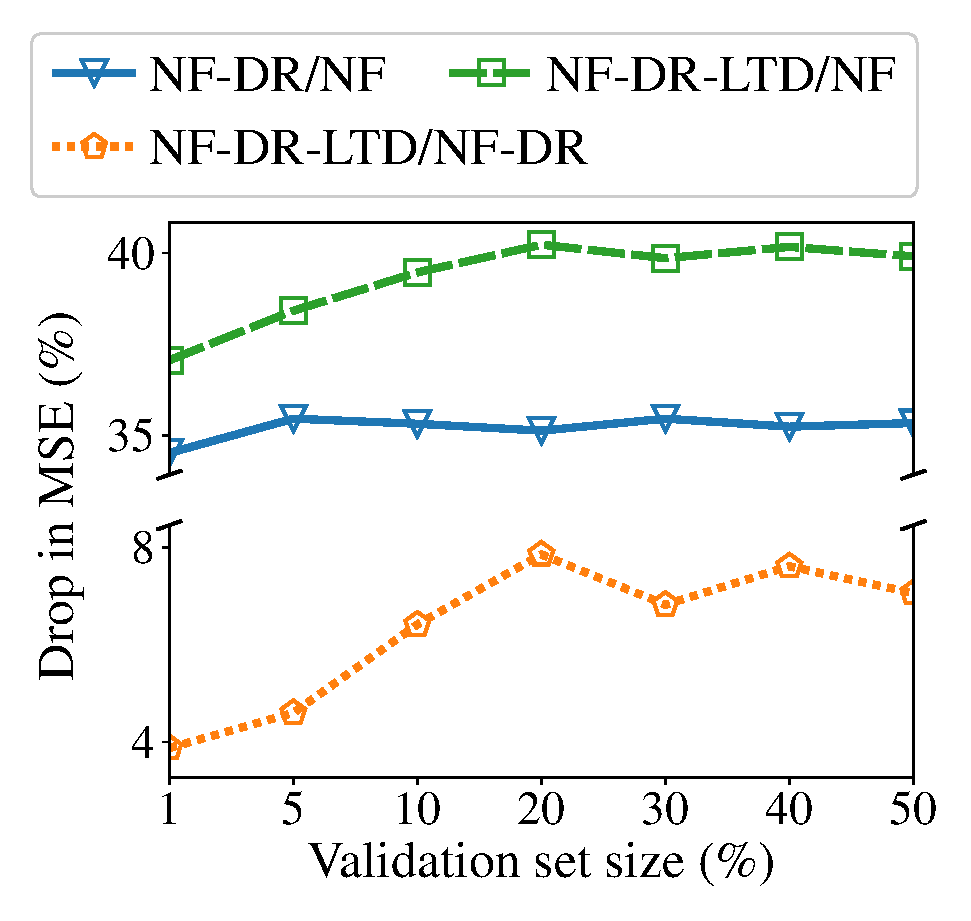
\includegraphics[height=3.88cm]{fig/drop_unbiased_size.eps}
  \caption{Comparing two approaches.}
  \label{fig:validation set comparison}
\end{subfigure}
\caption{Effects of varying the validation set size on \textsc{Music}.}
\end{figure}%
\end{minipage}
\end{figure}

Last, we study the trade-off between the validation set size and the inaccuracy of LTD.
We split the unbiased ratings into a fixed testing set (50\%) and a validation set with varying sizes (1\%-50\%).
We show the result by MSE on \textsc{Music} in Fig.~\ref{fig:validation set inaccuracy}.
We can see that LTD performs better as the validation set size increases because more observed ratings are used for training.
%to learn the rating and the propensity model.
% This suggests that a certain number of unbiased ratings are sufficient to learn a good propensity model.
We further explore the validation set size required to learn a good propensity model within LTD by computing the improvements between NF, NF-DR, and NF-DR-LTD.
We show the result in terms of percentage decrease in MSE on \textsc{Music} in Fig.~\ref{fig:validation set comparison}.
We can see that the improvements of NF-DR-LTD over NF and NF-DR grow when we vary the validation set size from 1\% to 20\%, but do not grow afterwards (the improvement over NF-DR is up to 7.9\% drop in MSE).
In contrast, the improvement of NF-DR over NF keeps steady because a small validation set can already fit the naive Bayes model well.

\section{Conclusions}
We proposed a novel approach, learning to debias (LTD), for training recommender systems on biased datasets.
To tackle two challenges in training the parameters of LTD, we developed a variance-regularized training algorithm.
We showed how to apply LTD to improve two-phase learning on four real-world datasets.
While the two-phase learning is vulnerable to the error and variance of propensity estimation, LTD achieves up to a 7.9\% drop in recommendation inaccuracy.
For future work, we will explore theoretical bounds on the generalization ability of a rating model trained by LTD.


{\clearpage\bibliographystyle{aaai}\bibliography{main}}


\appendix

\section{Additional Preliminaries}
\label{app:additional preliminaries}
Suppose we obtain partial observations of the true rating matrix  $\trueRatings$ in a certain way, either by allowing users to freely rate a fraction of items or by asking users to rate a number of randomly selected items.
We use $\trueRatings^\obsPairs$ and $\trueRatings^\misPairs$ to denote the observed and the missing ratings obtained this way, where $\obsPairs\cap\misPairs=\varnothing$ and $\obsPairs\cup\misPairs=\allPairs$.
We collect the Bernoulli variable $\observation$ for all user-item pairs into an observation indicator matrix $\observations=\{\observation|u,i\in\allPairs\}$.
We also collect the feature vector $\biasedFeatures$ for all user-item pairs into a feature tensor $\allFeatures=\{\biasedFeatures|u,i\in\allPairs\}$, which contains all features that affect the observation indicator matrix.
The observed ratings are \emph{unbiased} if and only if the missing ratings are missing at random (MAR).
Formally, MAR means that the probability of obtaining the observation indicator matrix only depends on the observed ratings, i.e., $p(\observations|\trueRatings,\allFeatures)=p(\observations|\trueRatings^{\obsBiasedPairs})$~\cite{marlin2007collaborative}.
The observed ratings are \emph{biased} if and only if the missing ratings are not MAR (NMAR).
A reason for MAR to fail in the context of recommendation is that the propensity of observing the true rating depends on the value of that true rating~\cite{marlin2009collaborative}.

% A naive Bayes model's parameters $\propensityParam=\{\nbObservation_\obsIndicator,\nbCondition_{\ratingScale|\obsIndicator},\nbRating_\ratingScale|\ratingScale=1,...,\nScale\}$ are learned by maximizing a likelihood function
% \begin{equation*}
% \max_{\propensityParam}\likelihood{NB}(\propensityParam)
% =\lrdense{\prod}{u,i\in\obsBiasedPairs}\nbObservation_\obsIndicator
% \lrdense{\prod}{u,i\in\misBiasedPairs}(1-\nbObservation_\obsIndicator)
% +\lrdense{\prod}{u,i\in\obsBiasedPairs}\nbCondition_{\biasedRating|\obsIndicator}
% +\lrdense{\prod}{u,i\in\obsUnbiasedPairs}\nbRating_{\biasedRating}.
% \end{equation*}%
% This likelihood function can be maximized in closed form
% \begin{equation*}
% \begin{aligned}
% \nbObservation_\obsIndicator
% &=\frac{|\obsBiasedPairs|}{|\obsBiasedPairs|+|\misBiasedPairs|}
% =\frac{|\obsBiasedPairs|}{\nUser\nItem},\\
% \nbCondition_{\ratingScale|\obsIndicator}
% &=\frac{
%   \sum_{u,i\in\obsBiasedPairs}\llbracket\biasedRating=\ratingScale\rrbracket
% }{|\obsBiasedPairs|}, \text{ and }\\
% \nbRating_{\ratingScale}
% &=\frac{
%   \sum_{u,i\in\obsUnbiasedPairs}\llbracket\biasedRating=\ratingScale\rrbracket
% }{|\obsUnbiasedPairs|}.\\
% \end{aligned}
% \end{equation*}%

% Recall that another type of propensity models is called a logistic regression model, and its parameters can be denoted by $\propensityParam=\{\lgWeight,\lgBias\}$.
% These parameters are learned by maximizing a likelihood function
% \begin{equation*}
% \max_{\propensityParam}\likelihood{LR}(\propensityParam)
% =\lrdense{\prod}{u,i\in\obsBiasedPairs}\propensityModel
% \lrdense{\prod}{u,i\in\misBiasedPairs}(1-\propensityModel).
% \end{equation*}%

\section{Additional Experiments}
\label{app:additional experiments}

\subsubsection{Settings}
The proposed LTD can employ a logistic regression or a neural propensity model for propensity estimation.
These two models can use both discrete and continuous features regarding observed ratings.
Specifically, on \textsc{Music}, \textsc{Coat}, \textsc{Book}, and \textsc{Movie}, these two models use the following features:
(1) The identity of a user and an item (discrete).
(2) The number of ratings given by a user and received by an item (continuous).
(3) The mean rating given by a user and received by an item (continuous).
(4) The true rating of a user to an item (continuous).
On \textsc{Coat}, these two models also use the following covariates as features:
(1) The gender of a user (discrete).
(2) The age group of a user (discrete).
(3) The location of a user (discrete).
(4) How much a user is interested in fashion (discrete).
(5) The gender of a coat (discrete).
(6) The jacket type of a coat (discrete).
(7) The color of a coat (discrete).
(8) Whether a coat is promoted on front page (discrete).
On \textsc{Movie}, these two models also use the following covariates as features:
(1) The gender of a user (discrete).
(2) The age group of a user (discrete).
(3) The occupation of a user (discrete).
(4) The zip code of a user (discrete).
(5) The genre(s) of a movie (discrete).
We represent all discrete features by one-hot encoding and normalize all continuous features, each of which is divided by the corresponding maximum value, between 0 and 1.

Two-phase learning approaches use a propensity model, which is pre-trained as follows:
(1) On \textsc{Coat} and \textsc{Movie}, a regularized logistic regression model is trained using all pairs of user and item covariates as features~\cite{schnabel2016recommendations}.
(2) Since \textsc{Music} and \textsc{Book} have neither user nor item covariates, a naive Bayes model is trained using the validation set, i.e., 5\% of the testing set~\cite{wang2019doubly}.

For the neural propensity model, we search the activation function in \{ReLU, sigmoid, tanh\}, search the size of layers in \{32, 64, 128, 256, 512\}, and search the size of embeddings in \{8, 16, 32, 64, 128\}.
We set the batch size to 128 on \textsc{Music} and \textsc{Coat}.
Since \textsc{Book} and \textsc{Movie} contain much more observed ratings than \textsc{Music} and \textsc{Coat}, we set the batch size to 1024 on \textsc{Book} and \textsc{Movie}.
We schedule the learning rate in \{0.001, 0.005, 0.01, 0.05\}.
To prevent overfitting, we apply L2 regularization on the parameters of the rating, the propensity, and the error model.
We tune the L2 regularization in \{0.01, 0.05, 0.5, 0.1\}.

\textsc{Music} and \textsc{Coat} do not provide rating time, whereas \textsc{Book} and \textsc{Movie} do.
To study how the proposed LTD generalizes over time, we split the biased ratings on \textsc{Book} and \textsc{Movie} into a training (90\%) and a testing (10\%) set by time.
We find that the results by a time split are consistent with those by a random split in Tables~\ref{tab:mse overall results},~\ref{tab:mse ablation studies},~\ref{tab:mae overall results},~and~\ref{tab:mae ablation studies}.

\subsubsection{Overall Results}
We evaluate an approach on the testing set over 10 different runs.
We show the result by MAE on \textsc{Music} and \textsc{Coat} in the left half of Table~\ref{tab:mae overall results}, where the testing set is unbiased.
We also show the result on \textsc{Book} and \textsc{Movie} in the right half of Table~\ref{tab:mae overall results}, where the testing set is biased.
We can see that the results by MAE are consistent with those by MSE in Table~\ref{tab:mse overall results}.
We also find that the improvements of the proposed LTD by MAE are not as significant as those by MSE in Table~\ref{tab:mse overall results}.
Our explanation is that instead of using absolute errors, LTD use square errors, which share a similar form to MSE, for training.

\begin{table}[h]
\small
\centering
% \setlength\tabcolsep{6.0pt}
\caption{Average MAE of all approaches over 10 different runs.}
\label{tab:mae overall results}
\begin{threeparttable}
\begin{tabular}{l|cc||cc}
\toprule
& \multicolumn{2}{c||}{Unbiased testing set} & \multicolumn{2}{c}{Biased testing set} \\
\cmidrule(rl){2-5}
Approach & \textsc{Music} & \textsc{Coat} & \textsc{Book} & \textsc{Movie} \\
\midrule
MF & 1.167 & 0.948 & 0.609 & 0.604 \\
NF & 1.034 & 0.919 & 0.571 & 0.587 \\
\midrule
CPT-V & 0.914 & 0.992 & 0.798 & 0.775 \\
PMF-NMAR & 1.190 & 0.910 & 0.595 & 0.601 \\
MF-IPS & 0.857 & 0.891 & 0.635 & 0.615 \\
NF-IPS & 0.842 & 0.863 & 0.582 & 0.591 \\
MF-DR & 0.793 & 0.807 & 0.601 & 0.601 \\
NF-DR & 0.782 & 0.784 & 0.562 & 0.581 \\
\midrule
MF-IPS-LTD & 0.836 & 0.827 & 0.600 & 0.591 \\
NF-IPS-LTD & 0.827 & 0.812 & 0.558 & 0.575 \\
MF-DR-LTD & 0.781 & 0.770 & 0.572 & 0.588 \\
NF-DR-LTD & \textbf{0.776} & \textbf{0.759} & \textbf{0.539} & \textbf{0.574} \\
\bottomrule
\end{tabular}
\begin{tablenotes}[flushleft]
\footnotesize
\item[*] The bottom four rows show the proposed approaches.
\end{tablenotes}
\end{threeparttable}
\end{table}

\subsubsection{Ablation Studies}
We implement the propensity model of NF-DR-LTD by a simple propensity (SP), a logistic regression (LR), or a neural propensity (NP) model.
The NP model has one, two, or three hidden layers NP-(1/2/3).
We show the result by MAE on the four datasets in Table~\ref{tab:mae ablation studies}.
We can see that the result by MAE is similar to that by MSE in Table~\ref{tab:mse ablation studies}.
% We also find that the results of other LTD approaches are similar to that of NF-DR-LTD.

\begin{table}[h]
\small
\centering
\caption{Average MAE of NF-DR-LTD over 10 different runs.}
\label{tab:mae ablation studies}
\begin{tabular}{l|l|cc||cc}
\toprule
% \multicolumn{2}{c|}{} & \multicolumn{2}{c||}{Unbiased testing set} & \multicolumn{2}{c}{Biased testing set} \\
% \cmidrule(rl){3-6}
\multicolumn{2}{c|}{Propensity model} & \textsc{Music} & \textsc{Coat} & \textsc{Book} & \textsc{Movie} \\
\midrule
\multirow{2}{*}{Existing} & SP & 0.812 & 0.784 & 0.632 & 0.611 \\
& LR & 0.791 & 0.774 & 0.589 & 0.590 \\
\midrule
\multirow{3}{*}{Proposed} & NP-1 & 0.782 & 0.761 & 0.562 & 0.580 \\
& NP-2 & \textbf{0.776} & \textbf{0.759} & \textbf{0.539} & \textbf{0.574} \\
& NP-3 & 0.784 & 0.763 & 0.570 & 0.585 \\
\bottomrule
\end{tabular}
\end{table}



\end{document}
